\documentclass{article}
\usepackage[T1]{fontenc}
\usepackage[utf8]{inputenc}
\usepackage[french]{babel}
\usepackage{algorithmeUTF8}
\usepackage{color}
\usepackage{array}
\usepackage{amsmath}
\usepackage{graphicx}
\usepackage{float}
\usepackage{booktabs}
\usepackage[margin=3cm]{geometry}
\usepackage{fancyhdr}
\usepackage{listings}
\usepackage[dvipsnames]{xcolor}
\usepackage{amsmath,amssymb,amsfonts,mathrsfs}
\usepackage{caption}
\usepackage{eurosym}
\usepackage{hyperref}
\usepackage{multirow}
\hypersetup{breaklinks=true}
\def\UrlBreaks{\do\/\do-\do?\do0}
\hypersetup{hidelinks}
\definecolor{mypink1}{rgb}{0.858, 0.188, 0.478}
\usepackage{minted}
\usepackage{xcolor}
\usepackage[colorlinks=true , linkbordercolor=white , linkcolor=blue]{hyperref}
\usemintedstyle{borland}
\newcommand{\HRule}{\rule{\linewidth}{0.5mm}}
\lstset{language=C++,
                basicstyle=\ttfamily,
                keywordstyle=\color{blue}\ttfamily,
                stringstyle=\color{red}\ttfamily,
                commentstyle=\color{green}\ttfamily,
                morecomment=[l][\color{magenta}]{\#}
}


\author{}
\date{Octobre 2019}

\pagestyle{fancy}
\fancyhead[L]{}

\begin{document}
\begin{titlepage}

\begin{figure}
    \centering
    
\includegraphics[width=7cm]{logo.jpg}
\end{figure}
\begin{center}
    \HRule \\[0.4cm]
{ \huge \bfseries Rapport de projet d'algorithmique}\\[0.4cm]
\HRule \\[0.5cm]
{\Large{Jeu Othello}\\
\vspace{2cm}}
{\large \makeatletter
\@date
\makeatother}
\end{center}

\vspace{6cm}
% Author and supervisor
\begin{minipage}{0.4\textwidth}
\begin{flushleft} \large
\emph{Auteurs:}\\
Mathias \textsc{VAN AUDENHOVE} \\
Lucas \textsc{WANNENMACHER} \\
Sipeng \textsc{ZHENG} \\
Maria-Bianca \textsc{ZUGRAVU} \\

\end{flushleft}
\end{minipage}
\begin{minipage}{0.4\textwidth}
\begin{flushright} \large
\emph{Enseignant:} \\
Nicolas \textsc{DELESTRE} \\
\end{flushright}
\end{minipage}
\end{titlepage}


\newpage
\tableofcontents
\newpage
\section{Introduction}
Dans le cadre de notre EC d'Algorithmique avancée et programmation C, nous avons du concevoir une version simplifiée du jeu Othello. Notre groupe était composé de quatre membres : Bianca, Lucas, Sipeng et Mathias.\\

La méthodologie de travail était imposée à suivre le modèle de Cycle en V : \\
\begin{itemize}
\item Analyse : spécification des TAD et Analyse Descendante
\item Conception préliminaire
\item Conception détaillée
\item Développement
\item Tests Unitaires
\end{itemize}\\

Ainsi, le planning de travail a été conforme à cette méthodologie. Pourtant, il a fallu plusieurs fois revenir aux phases précédentes pour corriger les différentes erreurs de cohérence (signatures des fonctions, dépéndance entre elles voir décomposition des fonctions trop complexes), pour rajouter d'autres opérations aux TADs nécessaires pour le développement. En effet, notre analyse descendante a évolué tout au long de notre projet. \\

Notre version d'othello devait comporter deux modes de jeu: l'option \textit{standard} (permettant de faire une partie contre une intelligence artificielle) et l'option \textit{tournoi} (versionpermettant à deux IA de jouer l'une contre l'autre). \\

L’interface homme machine est libre (mode texte simple, utilisationde la librairiencurses, utilisation d’une librairie graphique comme GTK, etc.).\\

\newpage

\section{Analyse Descendante}


\begin{figure}[h]
\caption{Analyse Descendante}
\centering
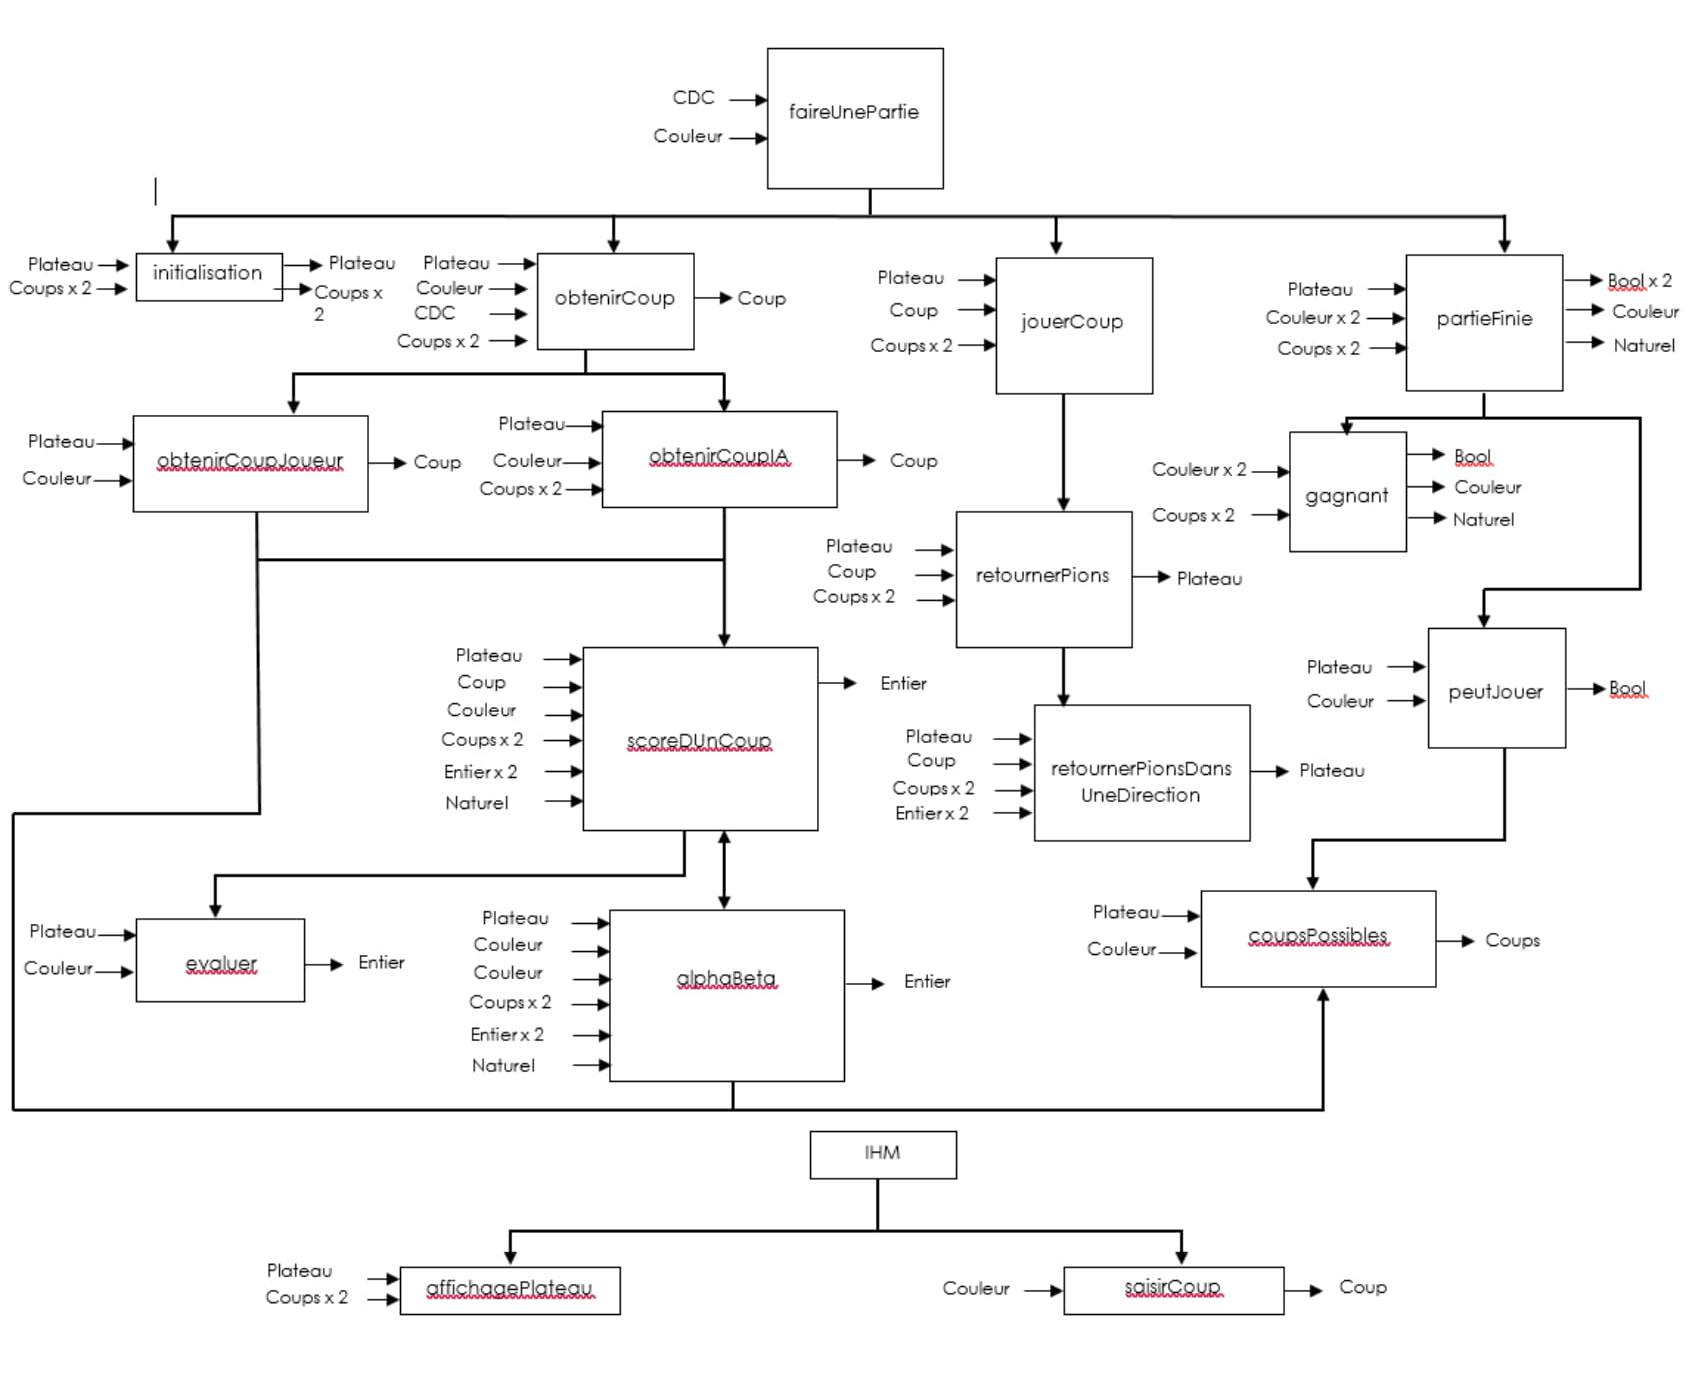
\includegraphics[width=1.1\textwidth]{analyseDescendante.jpg}
\end{figure}

\newpage
% ----------------------------------------------- TAD Couleur --------------------------------------------

\begin{tad}
\tadNom{Couleur}
\tadParametres{}
\tadDependances{}
\begin{tadOperations}{Couleur}
    \tadOperation{blanc}{}{\tadUnParam{Couleur}}
    \tadOperation{noir}{}{\tadUnParam{Couleur}}
    \tadOperation{changerCouleur}{\tadUnParam{Couleur}{}}{\tadUnParam{Couleur}}
\end{tadOperations}
\begin{tadSemantiques}{Couleur}
\tadSemantique{changerCouleur}{L’opération qui permet de changer la couleur}
\end{tadSemantiques}
\begin{tadAxiomes}
    \tadAxiome{changerCouleur(blanc) = noir}
    \tadAxiome{changerCouleur(noir) = blanc}
\end{tadAxiomes}
\end{tad} 
\begin{center}
 \HRule \\[0.4cm]   
\end{center}

% ------------------------------------------------- TAD PION -----------------------------------------------
\begin{tad}
\tadNom{Pion}
\tadParametres{}
\tadDependances{Couleur}
\begin{tadOperations}{Pion}
    \tadOperation{pion}{\tadUnParam{Couleur}{}}{\tadUnParam{Pion}}
    \tadOperation{obtenirCouleur}{\tadUnParam{Pion}{}}{\tadUnParam{Couleur}}
    \tadOperation{retournerPion}{\tadUnParam{Pion}{}}{\tadUnParam{Pion}}
\end{tadOperations}
\begin{tadSemantiques}{Couleur}
    \tadSemantique{obtenirCouleur}{L’opération qui permet d'obtenir la couleur d'un pion.}
    \tadSemantique{retournerPion}{L’opération qui permet de retourner un pion de l'adversaire, c'est à dire l'encadrer par deux pions à nous et de changer sa couleur. }
\end{tadSemantiques}
\begin{tadAxiomes}
    \tadAxiome{obtenirCouleur(pion(c)) = c}
    \tadAxiome{retournerPion(retournerPion(p)) = p}
\end{tadAxiomes}
\end{tad}
\begin{center}
 \HRule \\[0.4cm]   
\end{center}
% --------------------------------------------- TAD POSITION ------------------------------------------------
\begin{tad}
\tadNom{Position}
\tadParametres{}
\tadDependances{[\![1..8]\!], [\![a..h]\!]}
\begin{tadOperations}{Position}
    \tadOperation{position}{\tadDeuxParams{[\![1..8]\!]}{[\![a..h]\!]}}{\tadUnParam{Position}}
    \tadOperation{obtenirAbcisse}{\tadUnParam{Position}{}}{\tadUnParam{[\![1..8]\!]}}
    \tadOperation{obtenirOrdonnée}{\tadUnParam{Position}{}}{\tadUnParam{[\![a..h]\!]}}
\end{tadOperations}
\begin{tadSemantiques}{Position}
    \tadSemantique{obtenirAbcisse}{L’opération qui permet d'obtenir l'abcisse d'une position, c'est à dire la ligne sur laquelle on se positionne.}
    \tadSemantique{obtenirOrdonnée}{L’opération qui permet d'obtenir l'ordonnée d'une position, c'est à dire la colonne sur laquelle on se positionne.}
\end{tadSemantiques}
\begin{tadAxiomes}
    \tadAxiome{obtenirAbcisse(position(i,j)) = i où i $\in$ [\![1..8]\!]}
    \tadAxiome{obtenirOrdonnée(position(i,j)) = j où j $\in$ [\![a..h]\!]}
\end{tadAxiomes}
\end{tad}
\newpage
% -------------------------------------------- TAD PLATEAU ---------------------------------------------
\begin{tad}
\tadNom{Plateau}
\tadParametres{}
\tadDependances{Pion, Position, Booléen}
\begin{tadOperations}{Plateau}
    \tadOperation{plateau}{}{\tadUnParam{Plateau}}
    \tadOperationAvecPreconditions{poserPion}{\tadTroisParams{Pion}{Position}{Plateau}}{\tadUnParam{Plateau}}
    \tadOperationAvecPreconditions{enleverPion}{\tadDeuxParams{Position}{Plateau}}{\tadUnParam{Plateau}}
    \tadOperationAvecPreconditions{retournerPion}{\tadDeuxParams{Position}{Plateau}}{\tadUnParam{Plateau}}
    \tadOperationAvecPreconditions{obtenirPion}{\tadDeuxParams{Position}{Plateau}}{\tadUnParam{Pion}}
    \tadOperation{caseEstVide}{\tadDeuxParams{Position}{Plateau}}{\tadUnParam{Booléen}}
\end{tadOperations}
\begin{tadSemantiques}{Couleur}
    \tadSemantique{poserPion}{L’opération qui permet de poser un pion sur un plateau.}
    \tadSemantique{enleverPion}{L’opération qui permet d'enlever un pion depuis un plateau.}
    \tadSemantique{retournerPion}{L’opération qui permet de retourner un pion sur un plateau à partir de sa position.}
    \tadSemantique{obtenirPion}{L’opération qui permet d'obtenir un pion en fonction de sa position sur un plateau.}
    \tadSemantique{caseEstVide}{L’opération qui permet de vérifier si la case définie par une position sur le plateau est vide.}
\end{tadSemantiques}
\begin{tadPreconditions}{Plateau}
    \tadPrecondition{poserPion(p,pos,plateau)} \textit{caseEstVide(pos,plateau)}
    \tadPrecondition{enleverPion(pos,plateau)}  \textit{non(caseEstVide(pos,plateau))}
    \tadPrecondition{retournerPion(pos,plateau)} \textit{non(caseEstVide(pos,plateau))}
    \tadPrecondition{obtenirPion(pos,plateau)} \textit{non(caseEstVide(pos,plateau))}
\end{tadPreconditions}
\begin{tadAxiomes}
    \tadAxiome{obtenirPion(pos,poserPion(p,pos,plateau)) = p}
    \tadAxiome{retournerPion(pos,retournerPion(pos,plateau)) = plateau}
    \tadAxiome{caseEstVide(pos,plateau())}
    \tadAxiome{caseEstVide(pos,enleverPion(pos,plateau))}
    \tadAxiome{non caseEstVide(pos,poserPion(p,pos,plateau))}
\end{tadAxiomes}
\end{tad}
\begin{center}
 \HRule \\[0.4cm]   
\end{center}
% --------------------------------------------- TAD COUP -------------------------------------------------
\begin{tad}
\tadNom{Coup}
\tadParametres{}
\tadDependances{Pion, Position, Booléen}
\begin{tadOperations}{Coup}
    \tadOperation{coup}{\tadDeuxParams{Pion}{Position}}{\tadUnParam{Coup}}
    \tadOperation{obtenirPion}{\tadUnParam{Coup}{}}{\tadUnParam{Pion}}
    \tadOperation{obtenirPosition}{\tadUnParam{Coup}{}}{\tadUnParam{Position}}
    \tadOperation{estValide}{\tadUnParam{Coup}{}}{\tadUnParam{Booléen}}
\end{tadOperations}
\begin{tadSemantiques}{Coup}
    \tadSemantique{obtenirPion}{L’opération qui permet d'obtenir le pion correspondant à un coup.}
    \tadSemantique{obtenirPosition}{L’opération qui permet d'obtenir la position correspondante à un coup.}
    \tadSemantique{estValide}{L’opération qui permet de vérifier si un coup est valide, c'est à dire s'il n'est pas en dehors des limites du plateau.}
\end{tadSemantiques}
\begin{tadAxiomes}
    \tadAxiome{obtenirPion(coup(p,pos)) = p}
    \tadAxiome{obtenirPosition(coup(p,pos)) = pos}
\end{tadAxiomes}
\end{tad}

\newpage
% -------------------------------------- TAD COUPS -----------------------------------------------------------
\begin{tad}
\tadNom{Coups}
\tadParametres{Coup}
\tadDependances{Coup, Booléen, Naturel, NaturelNonNul}
\begin{tadOperations}{Coups}
    \tadOperation{coups}{}{\tadUnParam{Coups}}
    \tadOperation{estCoupValide}{\tadDeuxParams{Coups}{Coup}}{\tadUnParam{Booléen}}
    \tadOperationAvecPreconditions{iemeCoup}{\tadDeuxParams{Coups}{NaturelNonNul}}{\tadUnParam{Coup}}
    \tadOperation{ajouter}{\tadDeuxParams{Coups}{Coup}}{\tadUnParam{Coups}}
    \tadOperation{estPrésent}{\tadDeuxParams{Coups}{Coup}}{\tadUnParam{Booléen}}
    \tadOperation{nbCoups}{\tadUnParam{Coups}{}}{\tadUnParam{Naturel}}
\end{tadOperations}

\begin{tadSemantiques}{Coups}
    \tadSemantique{estCoupValide}{L’opération qui permet de vérifier qu'un coup est valide, c'est à dire s'il n'a pas été déjà fait et si sa position est conforme par rapports à celles d'autres pions y compris les pions adversaires.}
    \tadSemantique{iemeCoup}{L'opération qui permet d'obtenir l'ième coup.}
    \tadSemantique{ajouter}{L'opération qui permet d'ajouter un nouveau coup dans l'ensemble des coups.}
    \tadSemantique{estPrésent}{L'opération qui permet de vérifier si un coup a été déjà fait.}
    \tadSemantique{nbCoups}{L'opération qui permet de compter combien des coups on été faits en total.}
\end{tadSemantiques}
\begin{tadPreconditions}
    \tadPrecondition{iemeCoup(cps,i)} \textit{i $\leq$ nbCoups(cps)}
\end{tadPreconditions}
\begin{tadAxiomes}
    \tadAxiome{estCoupValable(cps,coup(p,pos))} \textit{ non estPrésent(cps,coup)} et \textit{estValide(coup)}
    \tadAxiome{ajouter(cps,coup)} \textit{nbCoups(cps) = nbCoups(cps) + 1}
    \tadAxiome{nbCoups(cps()) = 0}
    \tadAxiome{iemeCoup(ajouter(cps,coup),i) = coup}
\end{tadAxiomes}
\end{tad}
\newpage

\section{Conception préliminaire}

\subsection{Signatures des opérations de chaque TAD}
\subsubsection{TAD Couleur}
    \begin{algorithme}
        \signatureFonction{noir}{}{Couleur}
        \signatureFonction{blanc}{}{Couleur}
        \signatureProcedure{changerCouleur}{
            \paramEntreeSortie couleur : Couleur
            }
    \end{algorithme}
\subsubsection{TAD Pion}
    \begin{algorithme}
        \signatureFonction{pion}{Couleur}{Pion}
        \signatureFonction{obtenirCouleur}{Pion}{Couleur}
        \signatureProcedure{retournerPion}{
            \paramEntreeSortie pion : Pion
            }
    \end{algorithme}
\subsubsection{TAD Position}
    \begin{algorithme}
        \signatureFonction{position}{abcisse : [\![1..8]\!], coordonnee : [\![a..h]\!] }{Position}
        \signatureFonction{obtenirAbcisse}{Position}{[\![1..8]\!]}
        \signatureFonction{obtenirOrdonnee}{Position}{[\![a..h]\!]}
    \end{algorithme}
\subsubsection{TAD Plateau}
    \begin{algorithme}
        \signatureFonction{plateau}{}{Plateau}
        \signatureProcedureAvecPreconditions{poserPion}{
            \paramEntree unPion : Pion, pos : Position
            \paramEntreeSortie plateau : Plateau
            }{caseEstVide(pos, plateau)}
        \signatureProcedureAvecPreconditions{enleverPion}{
            \paramEntree pos : Position
            \paramEntreeSortie plateau : Plateau
            }{non(caseEstVide(pos, plateau))}
        \signatureProcedureAvecPreconditions{retournerPion}{
            \paramEntree pos : Position
            \paramEntreeSortie plateau : Plateau
            }{non(caseEstVide(pos, plateau))}
        \signatureFonctionAvecPreconditions{obtenirPion}{pos : Position, plateau : Plateau}{Pion}{non(caseEstVide(pos, plateau))}
        \signatureFonction{caseEstVide}{pos : Position, plateau : Plateau}{\booleen}
\end{algorithme}
\subsubsection{TAD Coup}
    \begin{algorithme}
        \signatureFonction{coup}{unPion : Pion, pos : Position}{Coup}
        \signatureFonction{obtenirPion}{unCoup : Coup}{Pion}
        \signatureFonction{obtenirPosition}{unCoup : Coup}{Position}
        \signatureFonction{estValide}{unCoup : Coup}{\booleen}
\end{algorithme}

\subsubsection{TAD Coups}
    \begin{algorithme}
        \signatureFonction{coups}{}{Coups}
        \signatureFonction{estCoupValide}{lesCoups : Coups, unCoup : Coup}{\booleen}
        \signatureFonctionAvecPreconditions{iemeCoup}{lesCoups: Coups, i : NaturelNonNul}{Coup}{i $\leq$ nbCoups(lesCoups)}
        \signatureProcedure{ajouter}{
        \paramEntreeSortie lesCoups: Coups
        \paramEntree unCoup : Coup
        }
        \signatureFonction{estPresent}{lesCoups : Coups, unCoup : Coup}{\booleen}
        \signatureFonction{nbCoups}{lesCoups : Coups}{Naturel}
    \end{algorithme}
    \subsection{Conception des TAD}
    Dans cette partie nous allons décrire comment sont représentés les TAD réperés lors de la phase d'analyse. La question la plus importante qui se pose c'est le choix entre une structure de données statique (tableau) et une structure de données dynamique (liste chainée ou arbre binaire) en fonction de nos besoins, tout en restant dans une compléxité gérable lors du dévéloppement en C.
    \subsubsection{TAD Couleur}
    Pour le \textbf{TAD Couleur} une représentation par une énumeration nous semble la plus efficace, étant donné que l'ensemble des valeurs d'une couleur est un ensemble dénombrable, discrèt: une couleur peut etre soit \textit{blanc} soit \textit{noir}. \\
    
    \textbf{typedef enum} Couleur \{BLANC,NOIR\} Couleur;
    \subsubsection{TAD Pion}
    Pour le \textbf{TAD Pion} une représentation par une structure contenant un seul champ (couleur) nous semble suffisant car, en effet, un pion se définit qu'à partir d'une couleur.
    \subsubsection{TAD Position}
    Pour le \textbf{TAD Position} une représentation par une structure contenant deux champs (abcisse et ordonnee) nous semble suffisant car, en effet, pour définir une position nous avons simplement besoin de l'indice de la ligne et de la colonne dans la grille..
    \subsubsection{TAD Plateau}
    Pour le \textbf{TAD Plateau} une représentation par une structure contenant un seul champ (cases) qui sera un dictionnaire ayant pour clés un tuple \textit{(x,y)} designant la position et comme valeur un pion nous semble la plus efficace. En effet, cette représentation nous facilitera le développement en ce qui concerne l'implémentation des opérations. Par example, pour l'opération \textit{obtenirPion} il nous suffira de retourner la valeur correspondante de la clé (une position), car ainsi nous aurons la valeur, soit le pion. De même, pour l'opération \textit{caseEstVide} il nous suffira de vérifier si la valeur retournée est un tuple vide ou pas. Pourtant, vu que nous allons dévélopper notre programme dans le langage C, ceci nous impose de laisser cette idée de côté pour le cas où nous serons en Python, car les dictionnaires sont difficile à conçevoir et à gérer en C.
    Enfin, nous avons choisi de faire une représentation par un tableau à deux dimensions.
    \subsubsection{TAD Coup}
    Pour le \textbf{TAD Coup} une représentation par une structure contenant deux champs (pion et position) nous semble suffisant car, en effet, à partir de cette représentation nous pourrons facilement obtenir un pion ou une position à partir d'un coup. De même, nous pourrons vérifier si un coup est valide simplement en vérifiant si la position où il devrait se positionner est déjà prise.
    \subsubsection{TAD Coups }
    Pour le \textbf{TAD Coups} une représentation par une structure contenant deux champs (lesCoups et nbCoups), où le premier champ sera une liste chainée nous semble la plus adéquate, car ce TAD est en fait un ensemble des coup avec un ordre (imposé par l'opération \textit{iemeCoup}). Pourtant, nous pouvons faire plus simple par représentant le premier champ par un tableau à une dimension.
    \newpage
    
 \subsection{Conception préliminaires des fonctions de l'Analyse Descendante}
    \subsubsection {Fonction initialiser}
        \begin{algorithme}
        \signatureFonction{initialiser}{plateau : Plateau, coupsJ1 : Coups, coupsJ2 : Coups}{plateau}
        \end{algorithme}
    \subsubsection {Procedure jouerCoup}
        \begin{algorithme}
        \signatureProcedure{jouerCoup}{plateau : Plateau, coup : Coup, coupsJ1 : Coups, coupsJ2 : Coups}
        \end{algorithme}
    \subsubsection {Fonction obtenirCoup}
        \begin{algorithme}
        \signatureFonction{obtenirCoup}{plateau : Plateau, couleur : Couleur, mode : $*$\caractere, coupsJ1 : Coups, coupsJ2 : Coups}{coup}
        \end{algorithme}
    \subsubsection {Fonction obtenirCoupIA}
        \begin{algorithme}
        \signatureFonction {evaluer}{plateau : Plateau, couleur : Couleur}{Entier}
        \signatureFonction {scoreDUnCoup}{plateau : Plateau, coup : Coup, couleur : Couleur, coupsJ1 : Coups, coupsJ2 : Coups, profondeur : Entier, alpha : Entier, beta : Entier}{Entier}
        \signatureFonction {alphaBeta}{plateau : Plateau, coup : Coup, joueurRef : Couleur, joueurCourant : Couleur, coupsJ1 : Coups, coupsJ2 : Coups, profondeur : Entier, alpha : Entier, beta : Entier}{Entier}
        \signatureFonction {obtenirCoupIA}{plateau : Plateau, couleur : Couleur, coupsJ1 : Coups, coupsJ2 : Coups}{Coup}
        \end{algorithme}
    \subsubsection {Fonction obtenirCoupJoueur}
        \begin{algorithme}
        \signatureFonction {obtenirCoupJoueur}{plateau : Plateau, joueurCourant : Couleur}{Coup}
        \end{algorithme}
    \subsubsection {Procedure retournerPions}
        \begin{algorithme}
        \signatureProcedure {retournerPionsDansUneDirection}{plateau : Plateau, coup : Coup, coupsJ1 : Coups, coupsJ2 : Coups, abscisse\_direction : \entier, ordonnee\_direction : \entier}
        \signatureProcedure {retournerPions}{plateau : Plateau, coup : Coup, coupsJ1 : Coups, coupsJ2 : Coups}
        \end{algorithme}
    \subsubsection {Fonction partieFinie}
        \begin {algorithme}
        \signatureFonction {gagnant}{joueur1 : Couleur, joueur2 : Couleur, coupsJ1 : Coups, coupsJ2 : Coups}{gagnant}
        \signatureFonction {partieFinie}{plateau : Plateau, coupsJ1 : Coups, coupsJ2 : Coups, joueur1 : Couleurs, joueur2 : Couleur}{PartieFinie}
        \end{algorithme}
    \subsubsection {Fonction coupsPossibles}
        \begin{algorithme}
        \signatureFonction {testCoup}{coup : Coup, plateau : Plateau}{Bouleen}
        \signatureFonction {coupPossible}{coup : Coup, plateau : Plateau}{Bouleen}
        \signatureFonction {coupsPossibles}{plateau : Plateau, couleurJoueur : Couleur}{Coups}
        \end{algorithme}
    \subsubsection {IHM}
        \begin{algorithme}
        \signatureProcedure {IHM\_affichagePlateau}{plateau : Plateau}
        \signatureFonction {IHM\_saisirCoup}{couleurJoueur : Couleur}{Coup}
        \end{algorithme}

    


\newpage
\section{Conception détaillée}

\subsection{faireUnePartie}

\subsection{obtenirCoup}
\begin{algorithme}
  \fonction{obtenirCoup}{plateau : $*$Plateau, joueurCourant : Couleur, mode : $*$\caractere, coupsJ1, coupsJ2 : Coups}{Coup}
           {
             coup : Coup\\
           }
           {
             \sialorssinon{mode$=$standard}
                          {
                            \sialorssinon{sontEgales(NOIR,joueurCourant)}
                                         {
                                           \affecter{coup}{obtenirCoupJoueur(plateau,joueurCourant)}
                                         }{
                                           \affecter{coup}{obtenirCoupIA(plateau,joueurCourant,coupsJ1,coupsJ2)}
                                         }
                          }{
                            \affecter{coup}{obtenirCoupIA(plateau,joueurCourant,coupsJ1,coupsJ2)}
                            \retourner{coup}
                          }
           }\\
\end{algorithme}



\subsubsection{obtenirCoupIA}

\begin{algorithme}
  \fonction{obtenirCoupIA}{plateau : $*$Plateau, couleur : Couleur, coupsJ1, coupsJ2 : Coups}{Coup}
           { cpsPossibles : Coups \\
             resultat : Coup \\
             score,alpha,beta,meilleurScore : \entier \\
             profondeur, i : \naturel \\
           }
           {
             \affecter{cpsPossibles}{coupsPossibles(plateau, couleur)}
             \affecter{resultat}{iemeCoup(cpsPossibles,1)}
             \affecter{alpha}{-1000}
             \affecter{beta}{1000}
             \affecter{profondeur}{3}
             \affecter{meilleurScore}{scoreDUnCoup(plateau,resultat,couleur,coupsJ1,coupsJ2,profondeur,alpha,beta)}
             \pour{i}{2}{nbCoups(cpsPossibles)}{}
                  {
                    \affecter{score}{scoreDUnCoup(plateau,iemeCoup(cpsPossibles,i),couleur,coupsJ1,coupsJ2,profondeur,alpha,beta)}
                    \sialors{score$>$meilleurScore}
                            {
                              \affecter{resultat}{iemeCoup(cpsPossibles,i)}
                              \affecter{meilleurScore}{score}
                            }
                    
                  }

             \retourner{resultat}
           }\\
           
\end{algorithme}

\begin{algorithme}
  \fonction{alphaBeta}{plateau : $*$Plateau, joueurRef, joueurCourant : Couleur, coupsJ1, coupsJ2 : Coups, profondeur : \naturel, alpha, beta : \entier}{\entier}
           { cpsPossibles : Coups \\
             score, resultat : \entier \\
             i : \naturel
           }
           {
             \affecter{cpsPossibles}{coupsPossibles(plateau, joueurCourant)}
             \sialors{nbCoups(cpsPossibles)$>$0}
                     {
                       \affecter{resultat}{scoreDUnCoup(plateau,iemeCoup(cpsPossibles,1),joueurRef,coupsJ1,coupsJ2,profondeur,alpha,beta)}
                     }
                     \pour{i}{2}{nbCoups(cpsPossibles)}{}
                          {
                            \affecter{score}{scoreDUnCoup(plateau,iemeCoup(cpsPossibles,i),joueurRef,coupsJ1,coupsJ2,profondeur,alpha,beta)}
                            \sialorssinon{joueurRef$=$joueurCourant}
                                         {
                                           \affecter{resultat}{min(score,resultat)}
                                           \sialors{resultat $<$ beta}
                                                   {
                                                     \affecter{beta}{resultat}
                                                     \sialors{alpha $>$ beta}
                                                             {
                                                               \retourner{resultat}
                                                             }
                                                   }
                                         }
                                         {
                                           \affecter{resultat}{max(score,resultat)}
				           \sialors{resultat $>$ alpha}
                                                   {
                                                     \affecter{alpha}{resultat}
                                                     \sialors{alpha $>$ beta}
                                                             {
                                                               \retourner{resultat}
                                                             }
                                                   }
                                         }
                          }
                          \retourner{resultat}
           }\\
\end{algorithme}

\begin{algorithme}
  \fonction{scoreDUnCoup}{plateau : $*$Plateau, coup : Coup, joueurRef : Couleur, coupsJ1, coupsJ2 : Coups, profondeur : \naturel, alpha, beta : \entier}{\entier}
           {
             copiePlateau : Plateau \\
           }
           {
             copier($@$copiePlateau,$*$plateau)\\
             jouerCoup($@$copiePlateau,coup,$@$coupsJ1,$@$coupsJ2)\\

             \sialorssinon{partieFinie($@$copiePlateau,coupsJ1,coupsJ2,joueurRef,changerCouleur(joueurRef)) OU profondeur$=$0}
                          {
                            \retourner{evaluer(copiePlateau,joueurRef)}
                          }
                          {
                            \retourner{alphaBeta($@$copiePlateau,joueurRef,changerCouleur(joueurRef),coupsJ1,coupsJ2,profonder$-$1,alpha,beta)}
                          }
           }\\
\end{algorithme}

\subsubsection{obtenirCoupJoueur}
\begin{algorithme}
  \fonction{obtenirCoupJoueur}{plateau : $*$Plateau, joueurCourant : Couleur}{Coup}
           {
             coup : Coup \\
             estCoupValide : \booleen
           }
           {
             \affecter{estCoupValide}{faux}
             \tantque{estCoupValide$=$faux}
                     {
                       \affecter{coup}{IHM\_saisirCoup(joueurCourant)}
                       \affecter{estCoupValide}{estPresent(coupsPossibles(plateau,joueurCourant),coup)}
                     }
                     \retourner{coup}
           }\\
\end{algorithme}


\subsection{partieFinie}

\begin{algorithme}
  \fonction{calculerScore}{coups : Coups}{\naturel}
           {
           }
           {
             \retourner{nbCoups(coups)}
           }\\
  
\end{algorithme}

\begin{algorithme}
  \fonction{peutJouer}{plateau : $*$Plateau, joueur : Couleur}{\booleen}
           {
           }
           {
             \retourner{nbCoups(coupsPossibles(plateau,joueur)$>$0)}
           }\\
\end{algorithme}

\begin{algorithme}
  \fonction{gagnant}{joueur1, joueur2 : Couleur, coupsJ1, coupsJ2 : Coups}{retourGagnant}
           {
             resultat : retourGagnant
           }
           {
             \affecter{resultat.couleurGagnant}{VIDE}
             \affecter{resultat.egalite}{faux}
             \affecter{resultat.scoreGagnant}{0}
             \sialorssinon{calculerScore(coupsJ1)$=$calculerScore(coupsJ2)}
                          {
                            \affecter{resultat.egalite}{vrai}
                            \affecter{resultat.scoreGagnant}{calculerScore(coupsJ1)}
                          }
                          {
                            \sialorssinon{calculerScore(coupsJ1)$<$calculerScore(coupsJ2)}
                                         {
                                           \affecter{resultat.egalite}{false}
                                           \affecter{resultat.couleurGagnant}{joueur2}
                                           \affecter{resultat.scoreGagnant}{calculerScore(coupsJ2)}
                                         }
                                         {
                                           \affecter{resultat.egalite}{false}
                                           \affecter{resultat.couleurGagnant}{joueur1}
                                           \affecter{resultat.scoreGagnant}{calculerScore(coupsJ1)}
                                         }
                          }
                          \retourner{resultat}
           }\\
\end{algorithme}
\begin{algorithme}
  \fonction{partieFinie}{plateau : $*$Plateau, coupsJ1,coupsJ2 : Coups, joueur1,joueur2 : Couleur}{retourPartieFinie}
           {
             resultat : retourPartieFinie\\
             rGagnant : retourGagnant\\
             partieFinie : \booleen
           }
           {
             \affecter{partieFinie}{faux}
             \sialorssinon{estRempli($*$plateau) OU (peutJouer(plateau,joueur1)=faux ET peutJouer(plateau,joueur2))}
                          {
                            \affecter{partieFinie}{vrai}
                            \affecter{rGagnant}{gagnant(joueur1,joueur2,coupsJ1,coupsJ2)}
                          }{
                            \affecter{rGagnant}{gagnant(joueur1,joueur2,coupsJ1,coupsJ2)}
                          }
                          \affecter{resultat.partieFinie}{partieFinie}
                          \affecter{resultat.couleurGagnant}{rGagnant.couleurGagnant}
                          \affecter{resultat.egalite}{rGagnant.egalite}
                          \affecter{resultat.scoreGagnant}{scoreGagnant}
                          \retourner{resultat}
           }\\
\end{algorithme}


\subsection{coupsPossibles}

\begin{algorithme}
  \fonction{testCoup}{coup : Coup, plateau : Plateau}{\booleen}
           {
             i,j,k,abscisse,ordonnee,newAbscisse,newOrdonnee : \entier\\
             couleurCaseATester, couleurJoueur : Couleur \\
             positionTestee : Position\\
             resultat : \booleen
           }
           {
             \affecter{couleurJoueur}{obtenirCouleur(obtenirPion(coup))}
             \affecter{resultat}{faux}
             \affecter{abscisse}{obtenirAbscisse(obtenirPosition(coup))}
             \affecter{ordonnee}{obtenirOrdonnee(obtenirPosition(coup))}
             \sialors{caseVide(plateau,obtenirPosition(coup))$=$vrai}
                     {
                       \affecter{i}{-1}
                       \tantque{i$<$2 ET resultat$=$faux}
                               {
                                 \affecter{j}{-1}
                                 \tantque{j$<$2 ET resultat$=$faux}
                                         {
                                             \sialors{(1\leq(abscisse$+$1)) ET ((abscisse$+$i)\leq8) ET (1\leq(ordonnee$+$j)) ET ((ordonnee+j)\leq8)}
                                         {
                                           \affecter{positionTestee}{position(abscisse$+$i,ordonne$+$j)}
                                           \sialors{caseVide(plateau,positionTestee)$=$faux}
                                                   {
                                                     \affecter{couleurCaseATester}{obtenirCouleur(obtenirPion(plateau,positionTestee))}
                                               
                                                   \sialors{sontEgales(couleurCaseATester,couleurJoueur)$=$faux}
                                                           {
                                                             \affecter{newAbscisse}{abscisse$+(2*i)$}
                                                             \affecter{newOrdonnee}{ordonnee$+2*j$}
                                                             \tantque{resultat$=$faux ET (1\leq newAbscisse) ET (newAbscisse\leq8) ET (1\leq newOrdonnee) ET (newOrdonnee\leq8) ET\\ caseVide(plateau,position(newAbscisse,newOrdonnee))}
                                                                     {
                                                                       \affecter{resultat}{sontEgales(obtenirCouleur(obtenirPion(plateau,\\position(newAbscisse,newOrdonnee))),couleurJoueur)}
                                                                       \affecter{k}{k+1}
                                                                       \affecter{newAbscisse}{newAbscisse$+$i}
                                                                       \affecter{newOrdonnee}{newOrdonne$+$j}
                                                                     }
                                                           }
                                         }
                                         }
                                         \affecter{j}{j$+$1}
                                         }
                                         \affecter{i}{i$+$1}
                               }
                     }
                     \retourner{resultat}
           }\\
\end{algorithme}

\begin{algorithme}
  \fonction{coupPossible}{coup : Coup, plateau: $*$Plateau}{\booleen}
           {
           }
           {
             \retourner{(estValide(coup) ET caseVide($*$plateau,obtenirPosition(coup)) ET testCoup(coup,$*$plateau))}
           }\\
\end{algorithme}

\begin{algorithme}
  \fonction{coupsPossibles}{plateau : $*$Plateau, couleurJoueur : Couleur}{Coups}
           {
             resultat : Coups\\
             i,j : \naturel\\
             coupAtester : Coup
           }
           {
             \pour{i}{1}{8}{}
                  {
                    \pour{j}{1}{8}{}
                         {
                           \affecter{coupAtester}{coup(pion(couleurJoueur),position(i,j))}
                           \sialors{coupPossible(coupAtester,plateau)}
                                   {
                                     ajouter($@$resultat,coupAtester)
                                   }
                         }
                  }
                  \retourner{resultat}
           }
\end{algorithme}








\newpage
\section{Gestion de projet}
\subsection{Suivi chronologique}
\begin{table}[h]
\centering
\begin{tabular}{|c|c|l|}
\hline
Séance                                                     & Date                                                              & Travail réalisé                                                                                                                                                  \\ \hline
1                                                          & 16/10/2019                                                        & Étude du sujet, mise en place de la gestion de projet
                                                                                          \\ \hline
2                                                          & 23/10/2019                                                        & Analyse : spécification des TAD  
                                                                                          \\ \hline
3                                                          & 6/11/2019                                                        & Analyse : analyse descendante 
                                                                                          \\ \hline
4                                                          & 13/11/2019                                                        & Conception préliminaire 
                                                                                          \\ \hline
5                                                          & 20/11/2019                                                        & Conception détaillée
                                                                                          \\ \hline
6                                                          & 27/11/2019                                                        & Développement 
                                                                                          \\ \hline
7                                                          & 4/12/2019                                                        & Développement et tests unitaires 
                                                                                          \\ \hline
8                                                          & 11/12/2019                                                        & Développement et tests unitaires
                                                                                          \\ \hline
9                                                          & Vacances de Noël                                                        & Développement et tests unitaires - Phase finale 
                                                                                          \\ \hline
10                                                          & 7/1/2020                                                        & Dépôt des livrables sur moodle 
                                                                                          \\ \hline
\end{tabular}
\end{table}

\textbf{La mise à jour du rapport a été faite tout au long de l'avancement.}

\subsection{Répartition des tâches}

\textbf{Signification des acronymes}
\begin{itemize}
  \item MVA : Mathias Van Audenhove
  \item LW : Lucas Wannenmacher
  \item SZ : Sipeng Zheng
  \item MBZ : Maria-Bianca Zugravu
\end{itemize}

\begin{table}[h]
\centering
\begin{tabular}{l|c|c|c|c|}

\cline{2-5}
                                                        & MVA & LW & SZ & MBZ \\ \hline
\multicolumn{1}{|l|}{Analyse descendante}               & X                     & X              & X                     & X                      \\ \hline
\multicolumn{1}{|l|}{README.txt}                        & \multicolumn{1}{l|}{} & X              & \multicolumn{1}{l|}{} & \multicolumn{1}{l|}{}  \\ \hline
\multicolumn{1}{|l|}{makefile}                          &                       & X               &                       & X                      \\ \hline
\multicolumn{1}{|l|}{Couleur.c}                         &                       &                &                       & X                      \\ \hline
\multicolumn{1}{|l|}{Pion.c}                            &                       &                &                       & X                      \\ \hline
\multicolumn{1}{|l|}{Position.c}                        &                       &                &                       & X                      \\ \hline
\multicolumn{1}{|l|}{Coup.c}                            &                       &                &                       & X                      \\ \hline
\multicolumn{1}{|l|}{Coups.c}                           &                       &                &                       & X                      \\ \hline
\multicolumn{1}{|l|}{Plateau.c}                         &                       &                &                       & X                      \\ \hline
\multicolumn{1}{|l|}{faireUnePartie.c}                  &                       &                &                       & X                       \\ \hline
\multicolumn{1}{|l|}{main.c}                  &                       &                &                       & X                       \\ \hline
\multicolumn{1}{|l|}{initialisation.c}                  & X                     &                &                       &                        \\ \hline
\multicolumn{1}{|l|}{jouerCoup.c}                       &                       & X               &                       &                        \\ \hline
\multicolumn{1}{|l|}{partieFinie.c}                     &                       &                &                       & X                      \\ \hline
\multicolumn{1}{|l|}{peutJouer}                         &                       &                &                       & X                      \\ \hline
\multicolumn{1}{|l|}{gagnant}                           &                       &                &                       & X                      \\ \hline
\end{tabular}
\end{table}

\newpage

\begin{table}[h]
\centering
\begin{tabular}{l|c|c|c|c|}

\cline{2-5}
& MVA & LW & SZ & MBZ \\ \hline
\multicolumn{1}{|l|}{calculerScore.c}                   &                       &                & X                     &                        \\ \hline
\multicolumn{1}{|l|}{obtenirCoup.c}                     &                       &                &                       & X                      \\ \hline
\multicolumn{1}{|l|}{obtenirCoupIA.c}                   &                       &                & X                     &                        \\ \hline
\multicolumn{1}{|l|}{alphaBeta}                         &                       &                & X                      & X                      \\ \hline
\multicolumn{1}{|l|}{scoreDUnCoup}                      &                       &                &                       & X                      \\ \hline
\multicolumn{1}{|l|}{evaluer}                           & X                      & X               &                       & X                      \\ \hline
\multicolumn{1}{|l|}{obtenirCoupJoueur.c}               &                       & X              &                       &                        \\ \hline
\multicolumn{1}{|l|}{coupsPossibles.c}                  & X                     &                &                       &                        \\ \hline
\multicolumn{1}{|l|}{testCoup}                          & X                     &                &                       &                        \\ \hline
\multicolumn{1}{|l|}{coupPossible}                      & X                     &                &                       &                        \\ \hline
\multicolumn{1}{|l|}{retournerPions.c}                  &                       & X              &                       &                        \\ \hline
\multicolumn{1}{|l|}{retournerPionsDansUneDirection}    &                       & X              &                       &                        \\ \hline
\multicolumn{1}{|l|}{IHM\_affichagePlateau}              &                       &                &                       & X                      \\ \hline
\multicolumn{1}{|l|}{IHM\_saisirCoup}                   &                       &                &                       & X                      \\ \hline
\multicolumn{1}{|l|}{Rapport}                           &                       &                &                       & X                      \\ \hline
\multicolumn{1}{|l|}{Rapport/Conclusion}                           & X                      &                &                       &                       \\ \hline
\multicolumn{1}{|l|}{Rapport/Conception préliminaire fonctions}                           & X                      &                &                       &                       \\ \hline
\multicolumn{1}{|l|}{Documentation}                     & X                      & X              &                       &                        \\ \hline
\multicolumn{1}{|l|}{testTADCouleur.c}                         &                       &                &                       & X                      \\ \hline
\multicolumn{1}{|l|}{testTADPion.c}                            &                       &                &                       & X                      \\ \hline
\multicolumn{1}{|l|}{testTADPosition.c}                        &                       &                &                       & X                      \\ \hline
\multicolumn{1}{|l|}{testTADCoup.c}                            &                       &                &                       & X                      \\ \hline
\multicolumn{1}{|l|}{testTADCoups.c}                           &                       &                &                       & X                      \\ \hline
\multicolumn{1}{|l|}{testTADPlateau.c}                         &                       &                &                       & X                      \\ \hline
\multicolumn{1}{|l|}{testCoupsPossibles.c}                     & X                     &                &                       &                        \\ \hline
\multicolumn{1}{|l|}{testJouerCoup.c}                          &                       & X              &                       &                        \\ \hline
\multicolumn{1}{|l|}{testRetournerPions.c}                     &                       & X              &                       &                        \\ \hline
\multicolumn{1}{|l|}{testRetournerPionsDansUneDirection.c}     &                       & X              &                       &                        \\ \hline
\multicolumn{1}{|l|}{testObtenirCoupIA.c}     &                       &               &                       & X                        \\ \hline
\multicolumn{1}{|l|}{testRetournerObtenirCoupJoueur.c}     &                       &               &                       & X                       \\ \hline
\end{tabular}
\end{table}
\newpage

\newpage
\section{Conclusion}

Ce projet nous a permis de mettre en application les notions théoriques que nous avons vu au cours du semestre. De plus, nous avons pu grace à lui nous familiariser avec l'outil de travil qu'est Git, que nous serons amenés à réutiliser à de nombreuses reprises au cours des prochaines années, et même dans notre vie professionnelle. En outre, la coordination entre les membres de l'équipe et la répartition du travail ne devaient pas être négligées. En effet, bien que nous ayons déjà été confrontés à ces problématiques de nombreuses fois au cours de notre scolarité, cette dernière prenait avec ce projet une tout autre dimension : l'utilisation de Git ou encore la rigueur qu'impose l'implémentation de fonctions, notamment dans le nom ou le type des variables, étaient pour nous de nouveaux enjeux. Ce fut donc une expérience enrichissante qui nous a permis de mieux situer les complexités inhérentes à la gestion d'un projet de groupe, dans le domaine de l'informatique plus particulièrement.\\

\textbf{Remarques personnelles}\\

\textit{Mathias Van Audenhove}\\

Personnellement, ce projet m'a apporté beaucoup d’expérience. J'avais certainement déjà les connaissances nécessaires à la conception logique de ce projet, mais je subissais encore des lacunes dans le domaine de l'implémentation. Ces dernières ont bien vite disparu. De plus, l'utilisation de Git et l'organisation d'un projet de groupe de cette envergure étaient également pour moi de nouveaux enjeux, avec lesquels j'ai pu me familiariser. Je le vois bien aujourd'hui : Au début de l'année, je n'avais pas la moindre idée concrète de la manière dont pouvait être géré un projet de ce genre. Aujourd'hui, et grâce à l'expérience acquise au cours de ce semestre, j'aborderai mes futurs projets confiant et en sachant quelles directions prendre pour les mener à bien.\\

\textit{Lucas Wannenmacher}\\

J'ai trouvé le projet très formateur, car il m'a permis non seulement de me perfectionner en C mais aussi d'apprendre à utiliser des outils tels que Git ou Doxygen (outils que j'ai d'ailleurs trouvé très pratiques) . Le projet a parfois demandé une une charge de travail relativement importante, notamment pour résoudre des bugs dont nous avions pris du temps à trouver l'origine. Le projet a aussi à mes yeux mis en évidence l'importance d'écrire ses fonctions et tests avec une certaine rigueur.\\

\textit{Sipeng Zheng}\\

Grâce à ce projet, j'ai pu améliorer mon travail en équipe, un aspect qui n'est pas aussi simple et évident que d'écrire du code de son côté. Chacun d'entre nous avait des idées différentes et le fait de se mettre d'accord sur les différents points, afin de bien se synchroniser pour le but commun du projet, peut être assez compliqué. De plus, l'outil Git nous a beaucoup facilité notre travail. Cela nous a permis de voir également le progrès des autres et de mieux collaborer.\\

\textit{Maria-Bianca Zugravu}\\

Grâce à ce projet, j'ai eu l'occasion de mettre en oeuvre les connaissances théoriques acquises dans cet EC et d'enrichir ces compétences. De même, en tant que chef de projet, j'ai découvert les différentes problématiques liées aux aspects organisationnels, tels que : la mise en oeuvre de la gestion de projet (le Git) afin de suivre en continu l'évolution et de prévoir les tâches à effectuer. Pourtant, ceci m'a posé des problèmes, le fait de synchroniser tout le monde et de s'assurer que chacun fait son travail n'a pas été tout à fait facile. En essayant de rester compréhensible et de maintenir une bonne ambiance au sein de l'équipe j'ai du accepter l'implication oscillante et parfois inexistante. Malgré tout cela, j'ai pu travailler en plus ce qui m'a permis d'apprendre beaucoup plus. 

\section{Bilan}

\begin{table}[h]
\centering
\begin{tabular}{|c|c|}
  \hline
Points accomplis                                                              & Améliorations                                                                                                                                                  \\ \hline
Première version fonctionnelle en mode standard/tournoi                                                              & Optimiser et passer à des versions plus stables                                                                                                                                                  \\ \hline
Affichage cohèrent et illustratif                                                              & \begin{tabular}[c]{@{}l@{}}Affichage graphique + intéractif (mode standard : \\indiquer les possibilités + nb des pions retournés)\end{tabular}                                                                                                                                                  \\ \hline
IA qui marche en utilisant alpha\-beta                                                              & \begin{tabular}[c]{@{}l@{}}Utiliser des algorithmes plus puissants\\($-$ de lenteur et taux de succès $+$ élevé) \end{tabular}                                                                                                                                                 \\ \hline
\begin{tabular}[c]{@{}l@{}}Utiliser au maximum les opérations des TAD\\ afin d'éviter de créer des nouvelles fonctions (Mise à jour)\end{tabular}                                                                     & Problème de portabilité     \\ \hline 
Tests unitaires pour chaque fonction (prèsque)                                                              & $+$ de tests afin de découvrir les bugs en amont                                                                                                                                                  \\ \hline
                                                              & $+$ plus de séances en équipe pour assurer l'implication                                                                                                                                                  \\ \hline
\end{tabular}
\end{table}


\newpage
\section{Code C}
\subsection{src}

\subsubsection{Couleur.c}
\begin{lstlisting}
/**
  * \file Couleur.c
  * \brief Conception du TAD Couleur
  * \author Maria Bianca Zugravu
  * \version 1.0
  * \date 01/12/2019
  */

#include "Couleur.h"

CLR_Couleur CLR_changerCouleur(CLR_Couleur couleur){
  if (couleur==BLANC)
    return NOIR;
  else
    return BLANC;
}

bool CLR_sontEgales(CLR_Couleur couleur1, CLR_Couleur couleur2){
  return (couleur1==couleur2);
}
\end{lstlisting}
  

\subsubsection{Pion.c}
\begin{lstlisting}
/**
 * \file Pion.c
 * \brief Implementation du TAD Pion
 * \author Maria Bianca Zugravu
 * \version 1.0
 */

#include <stdlib.h>
#include "Pion.h"

PION_Pion PION_pion(CLR_Couleur couleur) {
  PION_Pion pion;
  pion.couleur = couleur;
  return pion;

}

CLR_Couleur PION_obtenirCouleur(PION_Pion pion){
  return pion.couleur;
}

void PION_retournerPion(PION_Pion* pion){
  pion ->couleur= CLR_changerCouleur(PION_obtenirCouleur(*pion));
}

bool PION_sontEgaux(PION_Pion pion1, PION_Pion pion2){
  return CLR_sontEgales(pion1.couleur,pion2.couleur);
}
  
\end{lstlisting}

\subsubsection{Position.c}
\begin{lstlisting}
/**
 * \file Position.c
 * \brief Implementation du TAD position
 * \author Maria Bianca Zugravu
 * \version 1.0
 */

#include "Position.h"
#include <assert.h>

POS_Position POS_position(unsigned int abcisse, unsigned int ordonnee){
  assert(1<=abcisse);
  assert(abcisse<=8);
  assert(1<=ordonnee);
  assert(ordonnee<=8);
  POS_Position pos;
  pos.abcisse = abcisse;
  pos.ordonnee = ordonnee;
  return pos;
}

unsigned int POS_obtenirAbcisse(POS_Position pos){
  return pos.abcisse;
}

unsigned int POS_obtenirOrdonnee(POS_Position pos){
  return pos.ordonnee;
}

bool POS_sontEgales(POS_Position pos1, POS_Position pos2){
  return ((pos1.abcisse==pos2.abcisse) && (pos1.ordonnee==pos2.ordonnee));
}
  
\end{lstlisting}

\subsubsection{Coup.c}
\begin{lstlisting}
/**
 * \file Coup.c
 * \brief Implementation du TAD Coup
 * \author Maria Bianca Zugravu
 * \version 1.0
 */

#include "Coup.h"


COUP_Coup COUP_coup(PION_Pion pion, POS_Position pos){
  COUP_Coup coup;
  coup.pion = pion;
  coup.position = pos;
  return coup;
}

PION_Pion COUP_obtenirPion(COUP_Coup coup){
  return coup.pion;
}

POS_Position COUP_obtenirPosition(COUP_Coup coup){
  return coup.position;
}

bool COUP_estValide(COUP_Coup coup){
  /*fonction qui vérifie si le coup à placer ne sort pas des limites de la grille
   */
  return ((1<=POS_obtenirAbcisse(coup.position)) && (POS_obtenirOrdonnee(coup.position)<=8));
}

bool COUP_sontEgaux(COUP_Coup coup1, COUP_Coup coup2){
  return ((PION_sontEgaux(coup1.pion, coup2.pion))&&(POS_sontEgales(coup1.position,coup2.position)));

}
  
\end{lstlisting}

\subsubsection{Coups.c}
\begin{lstlisting}
/**
 * \file Coups.c
 * \brief Implementation du TAD Coups
 * \author Maria Bianca Zugravu
 * \version 1.0
 */

#include "Coups.h"
#include <assert.h>
#include <stdio.h>
#include <stdlib.h>


CPS_Coups CPS_coups(){
  CPS_Coups cps;
  cps.nbCoups=0;
  return cps;
}

void CPS_decalageVersLaGauche(CPS_Coups* coups, unsigned int indice){
  unsigned int i;
  for (i=indice;i<CPS_nbCoups(*coups);i++){
    (*coups).lesCoups[i]=(*coups).lesCoups[i+1];
  }
}
unsigned int CPS_obtenirIndiceDUnCoup(CPS_Coups coups, COUP_Coup coup){
  assert (CPS_estPresent(coups, coup));
  unsigned int indice=1;
  bool nonTrouve = false;
  while (!nonTrouve){
    nonTrouve=COUP_sontEgaux(CPS_iemeCoup(coups,indice),coup);
    indice++;
  }
  return (indice-1);
}

bool CPS_estPresent(CPS_Coups cps, COUP_Coup leCoup){
  bool estPresent=false;
  unsigned int i=0;
  while((i<NB_CPS_MAX) && (!estPresent)){
    if (COUP_sontEgaux(cps.lesCoups[i],leCoup))
      estPresent=true;
    i++;
  }
  return estPresent;
}
bool CPS_estCoupValide(CPS_Coups lesCoups, COUP_Coup leCoup){
  /* fonction qui vérifie que le coup n'est pas en dehors des limites du plateau
     et qu'il n'est pas été fait avant
   */
  return (COUP_estValide(leCoup) && !(CPS_estPresent(lesCoups,leCoup)));
}

COUP_Coup CPS_iemeCoup(CPS_Coups lesCoups, unsigned int i){
  return lesCoups.lesCoups[i];
}

void CPS_ajouter(CPS_Coups* lesCoups, COUP_Coup leCoup){
  if (!(CPS_estPresent(*lesCoups,leCoup))){
    (*lesCoups).nbCoups = (*lesCoups).nbCoups + 1;
    (*lesCoups).lesCoups[(*lesCoups).nbCoups] = leCoup;
  }
}

unsigned int CPS_nbCoups(CPS_Coups lesCoups){
  return lesCoups.nbCoups;
}

bool CPS_egal(CPS_Coups cps1, CPS_Coups cps2){
  bool egal;
  unsigned int i = 1;
  if (CPS_nbCoups(cps1)==CPS_nbCoups(cps2)) {
    egal = true;
    while (i<=CPS_nbCoups(cps1) && egal) {
      egal = COUP_sontEgaux(CPS_iemeCoup(cps1,i),CPS_iemeCoup(cps2,i));
      i++;
    }
  }else{
    egal = false;
  }
  return egal;  
}

void CPS_supprimer(CPS_Coups* coups, COUP_Coup coup){
  unsigned int indiceCoup;
  if (CPS_estPresent(*coups,coup)){
    indiceCoup = CPS_obtenirIndiceDUnCoup(*coups,coup);
    CPS_decalageVersLaGauche(coups,indiceCoup);
    (*coups).nbCoups = (*coups).nbCoups-1;
  }
}
  
\end{lstlisting}

\subsubsection{Plateau.c}
\begin{lstlisting}
/**
 * \file Plateau.c
 * \brief Implementation du TAD plateau
 * \author Maria Bianca Zugravu
 * \version 1.0
 */

#include <assert.h>
#include "Plateau.h"
#include <stdlib.h>


/* accesseurs */

void PL_fixerCaseAVide(PL_Plateau* plateau, POS_Position pos, bool estVide){
  (*plateau)[POS_obtenirAbcisse(pos)-1][POS_obtenirOrdonnee(pos)-1].caseVide=estVide;
}

void PL_fixerPionDansCase(PL_Plateau* plateau, POS_Position pos, PION_Pion pion){
  (*plateau)[POS_obtenirAbcisse(pos)-1][POS_obtenirOrdonnee(pos)-1].pion=pion;
}

void PL_initialiser(PL_Plateau* plateau){
  unsigned int i,j;
  for (i=1;i<=LARGEUR;i++){
    for (j=1;j<=HAUTEUR;j++){
      PL_fixerCaseAVide(plateau,POS_position(i,j),true);
    }
  }
}

bool PL_caseVide(PL_Plateau plateau, POS_Position pos){
  return plateau[POS_obtenirAbcisse(pos)-1][POS_obtenirOrdonnee(pos)-1].caseVide;
}

bool PL_estRempli(PL_Plateau plateau){
  unsigned int i, j, plateauRempli=true;
  POS_Position position;
  i=1; j=1;
  while ((plateauRempli)&&(i<=8)){
    j=1;
    while((plateauRempli)&&(j<=8)){
      position=POS_position(i,j);
      if (PL_caseVide(plateau,position))
	plateauRempli=false;
      j++;
    }
    i++;
  }
  return plateauRempli;
}

PION_Pion PL_obtenirPion(PL_Plateau plateau, POS_Position pos){
  assert(!PL_caseVide(plateau,pos));
  return plateau[POS_obtenirAbcisse(pos)-1][POS_obtenirOrdonnee(pos)-1].pion;
}

void PL_poserPion(PL_Plateau* plateau, POS_Position pos, PION_Pion pion){
  assert(PL_caseVide(*plateau,pos));
  PL_fixerPionDansCase(plateau,pos,pion);
  PL_fixerCaseAVide(plateau,pos,false);
}

void PL_enleverPion(PL_Plateau* plateau, POS_Position pos){
  assert (!PL_caseVide(*plateau,pos));
  PL_fixerCaseAVide(plateau,pos,true);
}

void PL_retournerPion(PL_Plateau* plateau,POS_Position pos){
  assert (!PL_caseVide(*plateau,pos));
  PION_Pion pion=PL_obtenirPion(*plateau,pos);
  PION_Pion* ppion;
  ppion=&pion;
  PION_retournerPion(ppion);
  PL_fixerPionDansCase(plateau,pos,*ppion);
  PL_fixerCaseAVide(plateau,pos,false);

}

bool PL_sontCasesEgales(PL_Plateau plateau1, PL_Plateau plateau2, POS_Position pos){
  if (!PL_caseVide(plateau1,pos) && !PL_caseVide(plateau2,pos)) {
    return PION_sontEgaux(PL_obtenirPion(plateau1,pos),PL_obtenirPion(plateau2,pos));
  } else {
    return PL_caseVide(plateau1,pos)==PL_caseVide(plateau2,pos);
  }
}

bool PL_sontPlateuxEgaux(PL_Plateau plateau1, PL_Plateau plateau2){
  unsigned int i,j;
  bool sontEgaux = true;
  i=1;j=1;
  while (i<=HAUTEUR && sontEgaux) {
    j=1;
    while (j<=LARGEUR && sontEgaux) {
      sontEgaux = PL_sontCasesEgales(plateau1,plateau2,POS_position(i,j));
      j++;
    }
    i++;
  }
  return sontEgaux;
}

void PL_copier(PL_Plateau* plateauCopie, PL_Plateau plateauSource){
  POS_Position pos;
  unsigned int i,j;
  for (i=1; i<=LARGEUR; i++) {
    for (j=1; j<=HAUTEUR; j++) {
      pos = POS_position(i,j);
      PL_fixerCaseAVide(plateauCopie,pos,PL_caseVide(plateauSource,pos));
      if (!PL_caseVide(plateauSource,pos)) {
        PL_fixerPionDansCase(plateauCopie,pos,PL_obtenirPion(plateauSource,pos));
      }
    }
  }
}
\end{lstlisting}

\subsubsection{coupsPossibles.c}
\begin{lstlisting}
/**
 * \file coupsPossibles.c
 * \brief fonction coupsPossibles
 * \version 1.0
 */

#include "coupsPossibles.h"


bool testCoup(COUP_Coup coup, PL_Plateau plateau){
    int i, j ,k;
    CLR_Couleur couleurCaseATester;
    CLR_Couleur couleurJoueur = PION_obtenirCouleur(COUP_obtenirPion(coup));
    POS_Position positionTestee;
    bool resultat = 0;
    int abscisse, ordonnee, newAbscisse, newOrdonnee;
    abscisse = POS_obtenirAbcisse(COUP_obtenirPosition(coup));
    ordonnee = POS_obtenirOrdonnee(COUP_obtenirPosition(coup));
    //On vérifie que la case à tester est bien vide.
    if (PL_caseVide(plateau,COUP_obtenirPosition(coup))){
        i = -1;
        //Pour chaque ligne.
        while ((i<2) && (resultat == 0)){
            j = -1;
            //Pour chaque colonne
            while ((j<2) && (resultat == 0)){
                //On va checker la case adjacente dans chaque direction.
                //Si les coordonnées de la case testée sont bien des coordonnées correctes, qui ne sortent pas des limites du plateau.
                if ((1<=abscisse+i) && (abscisse+i<=8) && (1<=ordonnee+j) && (ordonnee+j<=8)){
                    positionTestee = POS_position(abscisse + i, ordonnee + j);
                    //Si la case testée n'est pas vide.
                    if (!PL_caseVide(plateau, positionTestee)){
                        couleurCaseATester = PION_obtenirCouleur(PL_obtenirPion(plateau, positionTestee));
                        //Et enfin si la couleur de la case testée est celle de l'adversaire.
                        if (!CLR_sontEgales(couleurCaseATester, couleurJoueur)){
                            //Alors la case est valide : On commence la recherche dans cette direction.
                            newAbscisse = abscisse + 2*i;
                            newOrdonnee = ordonnee + 2*j;
                            //On check chaque case dans cette direction jusqu'à en trouver une qui valide ou invalide cette direction.
                            while ((!resultat) && (1<=newAbscisse) && (newAbscisse<=8) && (1<=newOrdonnee) && (newOrdonnee<=8) && (!PL_caseVide(plateau, POS_position(newAbscisse,newOrdonnee)))) {
                                resultat = (PION_obtenirCouleur(PL_obtenirPion(plateau, POS_position(newAbscisse,newOrdonnee))) == couleurJoueur);
                                //Si l'on trouve effectivement que cette case est un coup valide, alors on la sortie de la fonction doit être "vrai"
                                k++;
                                newAbscisse = newAbscisse + i;
                                newOrdonnee = newOrdonnee + j;
                            }
                        }
                    }
                }
                j++;
            }
            i++;
        }
    }
    return resultat;
}

bool coupPossible(COUP_Coup coup, PL_Plateau *plateau){
    return COUP_estValide(coup) && PL_caseVide(*plateau, COUP_obtenirPosition(coup)) && testCoup(coup, *plateau);
}

CPS_Coups coupsPossibles(PL_Plateau* plateau, CLR_Couleur couleurJoueur){
    CPS_Coups resultat = CPS_coups();
    int i,j;
    COUP_Coup CoupATester;

    for (i=1; i<9; i++){
        for (j=1; j<9; j++){
            CoupATester = COUP_coup(PION_pion(couleurJoueur), POS_position(i,j));
            if (coupPossible(CoupATester, plateau)){
                CPS_ajouter(&resultat, CoupATester);
            }
        }
    }
    return resultat;
}
  
\end{lstlisting}

\subsubsection{faireUnePartie.c}
\begin{lstlisting}
#include "faireUnePartie.h"


void faireUnePartie(char* mode, CLR_Couleur couleurChoisieHumain){
  PL_Plateau plateau;
  COUP_Coup coup1,coup2;
  CPS_Coups cps1 = CPS_coups();
  CPS_Coups cps2 = CPS_coups();
  CLR_Couleur joueur2;
  CLR_Couleur joueur1;
  bool fini = false;
  if (CLR_sontEgales(couleurChoisieHumain,NOIR)){
    joueur1 = couleurChoisieHumain;
    joueur2 = CLR_changerCouleur(joueur1);
  }else{
    joueur2 = couleurChoisieHumain;
    joueur1 = CLR_changerCouleur(joueur2);    
  }
  initialiser(&plateau, &cps1, &cps2);
  printf("\n\n ####################### OTHELLO ####################### \n\n");
  fflush(stdout);
  printf("\n\n >>>>>>>>>>>>>>>> Le jeu commence... \n\n");
  fflush(stdout);
  while (!partieFinie(&plateau,cps1,cps2,joueur1,joueur2).partieFinie && !fini){
    /* system("@cls||clear"); */
    printf("\n\n ####################### OTHELLO ####################### \n\n");
    fflush(stdout);
    IHM_affichagePlateau(plateau,cps1,cps2);
    printf("\n >>>>>>>>>>>>>>>> C'est aux NOIRS de jouer! \n");
    fflush(stdout);
    coup1 = obtenirCoup(&plateau,joueur1,mode,cps1,cps2);
    jouerCoup(&plateau,coup1,&cps1,&cps2);
    /* system("@cls||clear"); */
    IHM_affichagePlateau(plateau,cps1,cps2);
    printf("\n >>>>>>>>>>>>>>>> C'est aux BLANCS de jouer! \n");
    fflush(stdout);
    if(CPS_nbCoups(coupsPossibles(&plateau,joueur2))>0){
      coup2 = obtenirCoup(&plateau,joueur2,mode,cps1,cps2);
      jouerCoup(&plateau,coup2,&cps1,&cps2);
    }else{
      printf("\n >>>>>>>>>>>>>>>> Plus de coup possible! \n");
      fini = true;
    }
    /* system("@cls||clear"); */
  }
  if(partieFinie(&plateau,cps1,cps2,joueur1,joueur2).partieFinie || fini){
    IHM_affichagePlateau(plateau,cps1,cps2);
    printf("\n\n ####################### PARTIE FINIE  ####################### \n\n");
    fflush(stdout);
    if(partieFinie(&plateau,cps1,cps2,joueur1,joueur2).egalite){
      printf(" >>>>>>>>>>>>>>>> Il y a égalité :D \n");
      fflush(stdout);
    }else{
      if(CLR_sontEgales(partieFinie(&plateau,cps1,cps2,joueur1,joueur2).couleurGagnant,NOIR)){
	printf(" >>>>>>>>>>>>>>>> Les NOIRS ont gagné avec %d points !\n",partieFinie(&plateau,cps1,cps2,joueur1,joueur2).scoreGagnant);
	fflush(stdout);
      }else{
	printf(" >>>>>>>>>>>>>>>> Les BLANCS ont gagné avec %d points !\n",partieFinie(&plateau,cps1,cps2,joueur1,joueur2).scoreGagnant);
	fflush(stdout);
      }
    }
  }
}
\end{lstlisting}

\subsubsection{IHM.c}
\begin{lstlisting}
/**
 * \file IHM.c
 * \brief fonction IHM
 * \version 1.0
 */

#include "IHM.h"
#include <stdio.h>
#include <stdlib.h>
#include <string.h>

void IHM_affichagePlateau(PL_Plateau plateau, CPS_Coups coupsJ1, CPS_Coups coupsJ2){
  printf("\n");
  int i, j;
  printf("   a b c d e f g h [BLANCS=%d NOIRS=%d] \n", CPS_nbCoups(coupsJ2), CPS_nbCoups(coupsJ1));
  for(i=1;i<=LARGEUR;i++){
    printf("%d ",i);
    for(j=1;j<=HAUTEUR;j++){
      if (PL_caseVide(plateau,POS_position(i,j)))
	printf(" .");
      else{
	if (PION_obtenirCouleur(PL_obtenirPion(plateau,POS_position(i,j)))==NOIR)
	  printf(" x");
	else
	  printf(" o");
      }
    }
    printf("\n");
  }
}

COUP_Coup IHM_saisirCoup(CLR_Couleur couleurJoueur){
  COUP_Coup leCoup;
  char coup[5];
  while(!((1<=coup[1]-'0') && (coup[1]-'0'<=8) && (1<=(int)coup[0]-96) && ((int)coup[0]-96<=8) && (strlen(coup)==4))){
    printf("\n \n Veuillez entrer un coup (une lettre entre a et h, puis un chiffre entre 1 et 8 et enfin le caractère de retour '\\n'. Voici un exemple pour le coup e5 : 'e5\\n' ) : \n");
    fgets(coup,5*sizeof(char),stdin);
    int ch;
    while((ch = getchar()) != '\n' && ch != EOF);
  }
  leCoup = COUP_coup(PION_pion(couleurJoueur),POS_position(coup[1]-'0',(int)coup[0]-96));
  return leCoup;
}
\end{lstlisting}

\subsubsection{initialiser.c}
\begin{lstlisting}
/**
 * \file initialiser.c
 * \brief fonction initialiser
 * \version 1.0
 */

#include "initialiser.h"
#include "Plateau.h"
#include <stdlib.h>
#include "Position.h"
#include <stdbool.h>

void initialiser(PL_Plateau* plateau, CPS_Coups* coupsJ1, CPS_Coups* coupsJ2){
  PL_initialiser(plateau);
  PL_fixerPionDansCase(plateau, POS_position(4,4), PION_pion(BLANC));
  CPS_ajouter(coupsJ2, COUP_coup(PION_pion(BLANC), POS_position(4,4)));
  PL_fixerCaseAVide(plateau,POS_position(4,4),false);
  PL_fixerPionDansCase(plateau, POS_position(5,5), PION_pion(BLANC));
  CPS_ajouter(coupsJ2, COUP_coup(PION_pion(BLANC), POS_position(5,5)));
  PL_fixerCaseAVide(plateau,POS_position(5,5),false);
  PL_fixerPionDansCase(plateau, POS_position(4,5), PION_pion(NOIR));
  CPS_ajouter(coupsJ1, COUP_coup(PION_pion(NOIR), POS_position(4,5)));
  PL_fixerCaseAVide(plateau,POS_position(4,5),false);
  PL_fixerPionDansCase(plateau, POS_position(5,4), PION_pion(NOIR));
  CPS_ajouter(coupsJ1, COUP_coup(PION_pion(NOIR), POS_position(5,4)));
  PL_fixerCaseAVide(plateau,POS_position(5,4),false);
}
\end{lstlisting}

\subsubsection{jouerCoup.c}
\begin{lstlisting}
/**
 * \file jouerCoup.c
 * \brief Conception de jouerCoup
 * \author WANNENMACHER Lucas
 * \version 1.0
 * \date 01/12/2019
 */



#include "jouerCoup.h"



void jouerCoup(PL_Plateau *plateau, COUP_Coup coup, CPS_Coups* coupsJ1, CPS_Coups* coupsJ2){
  PL_poserPion(plateau,COUP_obtenirPosition(coup),COUP_obtenirPion(coup));
  if (PION_obtenirCouleur(COUP_obtenirPion(coup))==NOIR){
    CPS_ajouter(coupsJ1, coup);
  }else{
    CPS_ajouter(coupsJ2, coup);
  }
  retournerPions(plateau,coup, coupsJ1, coupsJ2);
}
\end{lstlisting}

\subsubsection{main.c}
\begin{lstlisting}
/**
 * \file main.c
 * \brief le main
 * \version 1.0
 */

#include <stdlib.h>
#include <stdio.h>
#include <string.h>
#include "faireUnePartie.h"

void othello_aide(){
  printf("Aide du programme othello \n");
  printf("Les options possibles sont : \n");
  printf("- standard blanc|noir [profondeur>2] : permet de jouer contre l'ordinateur en lui donnant les blancs ou les noirs (par défaut la profondeur est egale à 5)\n");
  printf("- tournoi blanc|noir [profondeur>2] : permet de faire confronter notre IA à elle-même (par défaut la profondeur est egale à 5)\n");
}


int main(int argc, char** argv){
  char* mode = argv[1];
  CLR_Couleur couleurJoueurHumain;
  if (argc==3 && (!strcmp(mode,"standard") || !strcmp(mode,"tournoi")) && (!strcmp(argv[2],"noir") || !strcmp(argv[2],"blanc"))){
    if (!strcmp(argv[2],"noir")){
      couleurJoueurHumain = NOIR;
    }else{
      couleurJoueurHumain = BLANC;
    }
    faireUnePartie(mode,couleurJoueurHumain);
  }else{
    othello_aide();
  }
  return EXIT\_SUCCESS;
}
 
\end{lstlisting}

\subsubsection{obtenirCoup.c}
\begin{lstlisting}
/**
 * \file obtenirCoup.c
 * \brief fonction obtenirCoup
 * \version 1.0
 */

#include "obtenirCoup.h"
#include <string.h>

COUP_Coup obtenirCoup(PL_Plateau* plateau, CLR_Couleur joueurCourant,char* mode,CPS_Coups cpsJ1, CPS_Coups cpsJ2){
  COUP_Coup coup;
  char* mode1 = "standard";
  CLR_Couleur noir = NOIR;
  if (strcmp(mode,mode1)==0){
    if (CLR_sontEgales(noir,joueurCourant)){
      coup = obtenirCoupJoueur(plateau,joueurCourant);
    }else{
      coup = obtenirCoupIA(plateau,joueurCourant,cpsJ1,cpsJ2);
      printf("Coup IA (%x,%x) :", POS_obtenirAbcisse(COUP_obtenirPosition(coup)), POS_obtenirOrdonnee(COUP_obtenirPosition(coup)));
    }
  }
  else{
    coup = obtenirCoupIA(plateau,joueurCourant,cpsJ1,cpsJ2);
  }
  return coup;
}
\end{lstlisting}

\subsubsection{obtenirCoupIA.c}
\begin{lstlisting}
/**
 * \file obtenirCoupIA.c
 * \brief fonction obtenirCoupIA
 * \version 1.0
 */

#include "obtenirCoupIA.h"
#include <stdlib.h>
#include <stdio.h>

int max(int a, int b){
  if (a>b)
    return a;
  else
    return b;
}

int min(int a, int b){
  if (a<b)
    return a;
  else
    return b;
}

int signe(int a){
  return a/abs(a);
}

int evaluer(PL_Plateau plateau, CLR_Couleur joueur){
  int matriceValeurCases[8][8] = {{1000,-200,50,12,12,50,-200,1000},
			   {-200,-400,0,0,0,0,-400,-200},
			   {50,0,5,1,1,5,0,50},
			   {12,0,1,10,10,1,0,12},
			   {12,0,1,10,10,1,0,12},
			   {50,0,5,1,1,5,0,50},
			   {-200,-400,0,0,0,0,-400,-200},
			   {1000,-200,50,12,12,50,-200,1000}};
  unsigned int i, j;
  PION_Pion pion = PION_pion(joueur);
  POS_Position pos, posCoin;
  int scoreJoueur = 0;
  for (i=1;i<=LARGEUR;i++){
    for (j=1;j<=HAUTEUR;j++){
      pos = POS_position(i,j);
      if (!PL_caseVide(plateau, pos)){
        if (PION_sontEgaux(PL_obtenirPion(plateau,pos),pion)){
          if ((i==2 || i==7) && (j==2 || j==7)){
            posCoin = POS_position(i+signe(i-4), j+signe(j-4));
            //posCoin = POS_position(i+((i-4)/abs(i-4)), j+((j-4)/abs(j-4)));
            if (!PL_caseVide(plateau,posCoin)){
              if (PION_sontEgaux(PL_obtenirPion(plateau, posCoin),pion)){
                scoreJoueur = scoreJoueur + 100;
              }
            }
          }
          else{
            scoreJoueur = scoreJoueur + matriceValeurCases[i-1][j-1];
          }
        }
      }      
    }
  }
  return scoreJoueur;
}

int scoreDUnCoup(PL_Plateau* plateau, COUP_Coup coup, CLR_Couleur joueurRef,CPS_Coups coupsJ1, CPS_Coups coupsJ2, unsigned int profondeur, int alpha, int beta){
  PL_Plateau copiePlateau;
  PL_copier(&copiePlateau,*plateau);
  jouerCoup(&copiePlateau,coup,&coupsJ1,&coupsJ2);
  if ((partieFinie(&copiePlateau,coupsJ1,coupsJ2,joueurRef,CLR_changerCouleur(joueurRef)).partieFinie) || (profondeur==0)){
    return evaluer(copiePlateau,joueurRef);
  }else{
    return alphaBeta(&copiePlateau,joueurRef, CLR_changerCouleur(joueurRef),coupsJ1,coupsJ2,profondeur-1,alpha,beta);
  }
}

int alphaBeta(PL_Plateau* plateau, CLR_Couleur joueurRef, CLR_Couleur joueurCourant,CPS_Coups coupsJ1, CPS_Coups coupsJ2, unsigned int profondeur, int alpha, int beta){
  CPS_Coups cpsPossibles = coupsPossibles(plateau,joueurCourant);
  int resultat,score;
  unsigned int i;
  if (CPS_nbCoups(cpsPossibles)>0){
    resultat = scoreDUnCoup(plateau,CPS_iemeCoup(cpsPossibles,1),joueurRef, coupsJ1, coupsJ2,profondeur,alpha,beta);
  }
  for (i=2;i<=CPS_nbCoups(cpsPossibles);i++){
    score = scoreDUnCoup(plateau,CPS_iemeCoup(cpsPossibles,i), joueurRef,coupsJ1,coupsJ2,profondeur,alpha,beta);
    /* cas du joueur à minimiser */
    if (joueurRef==joueurCourant){
      resultat = min(score,resultat);
      if (resultat<beta){
	beta = resultat;
	/* condition pour traiter que les branches intéressantes de l'arbre*/
	if (alpha>beta){
	  return resultat;
	}
      }
    }
    /* cas du joueur à maximiser */
    else{
      resultat = max(score,resultat);
      if (resultat>alpha){
	alpha=resultat;
	if (alpha>beta){
	  return resultat;
	}
      }
    }
  }
  return resultat;
}

COUP_Coup obtenirCoupIA(PL_Plateau* plateau, CLR_Couleur couleur, CPS_Coups coupsJ1, CPS_Coups coupsJ2){
  CPS_Coups cpsPossibles = coupsPossibles(plateau, couleur);
  COUP_Coup resultat = CPS_iemeCoup(cpsPossibles,1);
  int score;
  int alpha = -1000;
  int beta = 1000;
  unsigned int profondeur = 5; 
  int meilleurScore = scoreDUnCoup(plateau,resultat,couleur, coupsJ1, coupsJ2,profondeur,alpha,beta);
  for (unsigned int i=2;i<=CPS_nbCoups(cpsPossibles);i++){
    score = scoreDUnCoup(plateau,CPS_iemeCoup(cpsPossibles,i),couleur,coupsJ1, coupsJ2,profondeur,alpha,beta);
    if (score>meilleurScore){
      resultat = CPS_iemeCoup(cpsPossibles,i);
      meilleurScore = score;
    }
  }
  return resultat;
}
\end{lstlisting}

\subsubsection{obtenirCoupJoueur.c}
\begin{lstlisting}
/**
 * \file obtenirCoupJoueur.h
 * \brief fonction obtenirCoupJoueur
 * \version 1.0
 */

#include "obtenirCoupJoueur.h"
#include "Couleur.h"
#include <stdbool.h>

COUP_Coup obtenirCoupJoueur(PL_Plateau* plateau, CLR_Couleur joueurCourant){
  bool estCoupValide = false;
  COUP_Coup coup;
  while (!estCoupValide){
    coup = IHM_saisirCoup(joueurCourant);
    estCoupValide = CPS_estPresent(coupsPossibles(plateau,joueurCourant),coup);
  }
  return coup;
}
\end{lstlisting}

\subsubsection{partieFinie.c}
\begin{lstlisting}
/**
 * \file partieFinie.c
 * \brief fonction partieFinie
 * \version 1.0
 */

#include "partieFinie.h"

typedef struct GAGNANT_retour{
  CLR_Couleur couleurGagnant;
  bool egalite;
  unsigned int scoreGagnant;
}GAGNANT_retour;

unsigned int calculerScore(CPS_Coups coups){
  return CPS_nbCoups(coups);
}

bool peutJouer(PL_Plateau* plateau, CLR_Couleur joueur){
  return CPS_nbCoups(coupsPossibles(plateau, joueur)) > 0;
}

GAGNANT_retour gagnant(CLR_Couleur joueur1, CLR_Couleur joueur2, CPS_Coups coupsJ1, CPS_Coups coupsJ2){
  GAGNANT_retour resultat;
  resultat.couleurGagnant = VIDE;
  resultat.egalite = false;
  resultat.scoreGagnant = 0;
  if (calculerScore(coupsJ1) == calculerScore(coupsJ2)){
    resultat.egalite = true;
    resultat.scoreGagnant = calculerScore(coupsJ1);
  } else {
    if (calculerScore(coupsJ1)<calculerScore(coupsJ2) ){
      resultat.egalite = false;
      resultat.couleurGagnant = joueur2;
      resultat.scoreGagnant = calculerScore(coupsJ2);
    }else {
      resultat.egalite = false;
      resultat.couleurGagnant = joueur1;
      resultat.scoreGagnant = calculerScore(coupsJ1);      
    }
  }    
  return resultat;  
}

PF_retour partieFinie(PL_Plateau* plateau,CPS_Coups coupsJ1,CPS_Coups coupsJ2,CLR_Couleur joueur1,CLR_Couleur joueur2){
  PF_retour resultat;
  GAGNANT_retour rGagnant;
  bool partieFinie;
  partieFinie=false;
  if ((PL_estRempli(*plateau))||(!(peutJouer(plateau,joueur1))&&(!(peutJouer(plateau,joueur2))))){
    partieFinie=true;
    rGagnant=gagnant(joueur1,joueur2, coupsJ1,coupsJ2);
  }else{
    rGagnant=gagnant(joueur1,joueur2,coupsJ1,coupsJ2);
  }
  resultat.partieFinie=partieFinie;
  resultat.couleurGagnant=rGagnant.couleurGagnant;
  resultat.egalite=rGagnant.egalite;
  resultat.scoreGagnant=rGagnant.scoreGagnant;
  return resultat;
}
\end{lstlisting}

\subsubsection{retournerPions.c}
\begin{lstlisting}
/**
 * \file retournerPions.c
 * \brief procedure qui retourne les pions a retourner
 * \author WANNENMACHER Lucas
 */

#include "retournerPions.h"
#include <stdio.h>
#include <stdbool.h>

/* cette fonction retourne les pions à retourner dans une direction */

void retournerPionsDansUneDirection(PL_Plateau* plateau,COUP_Coup coup, CPS_Coups* coupsJ1, CPS_Coups* coupsJ2,int abscisse_direction, int ordonnee_direction){
  CLR_Couleur couleurCoup = PION_obtenirCouleur(COUP_obtenirPion(coup));
  CLR_Couleur couleurOpposee = CLR_changerCouleur(couleurCoup);
  int n = 0; //n représente le nombre de cases à retourner
  bool deja_retourne = false; //ce booleen sert à ne pas retourner plusieurs fois le meme pion
  bool a_croise_case_vide = false; //ce booleen sert à ecarter le cas où il croise une case vide
  POS_Position PosCoup = COUP_obtenirPosition(coup);
  POS_Position PosCase = PosCoup;
  while(((POS_obtenirAbcisse(PosCase)+abscisse_direction)>0)&&((POS_obtenirAbcisse(PosCase)+abscisse_direction)<9)&&((POS_obtenirOrdonnee(PosCase)+ordonnee_direction)>0)&&((POS_obtenirOrdonnee(PosCase)+ordonnee_direction)<9)&&(!deja_retourne)&&(!a_croise_case_vide)){
    PosCase = POS_position(POS_obtenirAbcisse(PosCase)+abscisse_direction,POS_obtenirOrdonnee(PosCase)+ordonnee_direction);
    if(PL_caseVide(*plateau,PosCase)){
      a_croise_case_vide = true;
    }
    else{
      if(PION_obtenirCouleur(PL_obtenirPion(*plateau,PosCase))==couleurOpposee){
	n++;
      }
      //si le prochain pion est de la couleur du pion posé, alors on retourne les pions entre ces deux pions
      if((PION_obtenirCouleur(PL_obtenirPion(*plateau,PosCase))==couleurCoup)){
        deja_retourne = true;
        if(n>0){
        for(int i = 1;i<=n;i++){
          PL_retournerPion(plateau,POS_position(POS_obtenirAbcisse(PosCoup)+i*abscisse_direction,POS_obtenirOrdonnee(PosCoup)+i*ordonnee_direction));
	  if (CLR_sontEgales(couleurCoup,NOIR)){
	    CPS_ajouter(coupsJ1, COUP_coup(PION_pion(couleurCoup), POS_position(POS_obtenirAbcisse(PosCoup)+i*abscisse_direction,POS_obtenirOrdonnee(PosCoup)+i*ordonnee_direction)));
	    CPS_supprimer(coupsJ2, COUP_coup(PION_pion(couleurOpposee),POS_position(POS_obtenirAbcisse(PosCoup)+i*abscisse_direction,POS_obtenirOrdonnee(PosCoup)+i*ordonnee_direction)));
	}else{
	    CPS_ajouter(coupsJ2, COUP_coup(PION_pion(couleurCoup), POS_position(POS_obtenirAbcisse(PosCoup)+i*abscisse_direction,POS_obtenirOrdonnee(PosCoup)+i*ordonnee_direction)));
	    CPS_supprimer(coupsJ1, COUP_coup(PION_pion(couleurOpposee),POS_position(POS_obtenirAbcisse(PosCoup)+i*abscisse_direction,POS_obtenirOrdonnee(PosCoup)+i*ordonnee_direction)));
	  }
	}
    }
  }
  }
  }
}


//cette procedure fait des appels de retournerPionsDansUneDirection pour chaque direction
void retournerPions(PL_Plateau *plateau,COUP_Coup coup, CPS_Coups* coupsJ1, CPS_Coups* coupsJ2){
  retournerPionsDansUneDirection(plateau,coup,coupsJ1,coupsJ2,1,0);
  retournerPionsDansUneDirection(plateau,coup,coupsJ1,coupsJ2,0,1);
  retournerPionsDansUneDirection(plateau,coup,coupsJ1,coupsJ2,-1,0);
  retournerPionsDansUneDirection(plateau,coup,coupsJ1,coupsJ2,0,-1);

  retournerPionsDansUneDirection(plateau,coup,coupsJ1,coupsJ2,1,1);
  retournerPionsDansUneDirection(plateau,coup,coupsJ1,coupsJ2,1,-1);
  retournerPionsDansUneDirection(plateau,coup,coupsJ1,coupsJ2,-1,-1);
  retournerPionsDansUneDirection(plateau,coup,coupsJ1,coupsJ2,-1,1);

}
\end{lstlisting}

\subsection{include}
\subsection{Couleur.h}
\begin{lstlisting}
/**
  * \file Couleur.h
  * \brief TAD couleur
  * \author Maria-Biancia Zugravu
  * \version 1.0
  * \date 01/12/2019
  */

#ifndef __COULEUR__
#define __COULEUR__

#include <stdbool.h>

/**
* \enum CLR_Couleur Couleur.h "include/Couleur.h"
* \brief il y a dans l'énumération les différentes couleurs d'un pion, sachant qu'un pion peut être de couleur 'VIDE'
* \author Maria-Biancia Zugravu
*/

typedef enum CLR_Couleur {BLANC,NOIR,VIDE} CLR_Couleur;

/**
* \fn CLR_Couleur CLR_changerCouleur(CLR_Couleur couleur)
* \brief renvoie la couleur inverse de celle en entrée (l'inverse de NOIR et BLANC et inversement)
* \author Maria-Biancia Zugravu
* \param couleur la couleur dont on veut l'inverse
* \return CLR_Couleur
*/

CLR_Couleur CLR_changerCouleur(CLR_Couleur);

/**
* \fn bool CL_changerCouleur(CLR_Couleur couleur1,CLR_Couleur couleur1)
* \brief rretourne vrai si les couleurs sont égals,faux sinon
* \author Maria-Biancia Zugravu
* \param couleur1 couleur2 les couleurs qui sont à comparer
* \return bool
*/
bool CLR_sontEgales(CLR_Couleur, CLR_Couleur);

#endif
\end{lstlisting}

\subsection{Pion.h}
\begin{lstlisting}
/**
  * \file Pion.h
  * \brief TAD pion fichier.h
  * \author Maria Bianca Zugravu
  * \version 1.0
  */

#ifndef __PION__
#define __PION__

#include "Couleur.h"

/**
* \struct PION_Pion Pion.h "include/Pion.h"
* \brief la structure representant un pion
* \author Maria Bianca Zugravu
*/

typedef struct PION_Pion{
  CLR_Couleur couleur;
} PION_Pion;

/**
* \fn PION_Pion PION_pion(CLR_Couleur)
* \brief retourne un pion de la couleur souhaitee
* \author Maria Bianca Zugravu
* \return PION_Pion
*/

PION_Pion PION_pion(CLR_Couleur);

/**
* \fn CLR_Couleur PION_obtenirCouleur(PION_Pion)
* \brief retourne la couleur d'un pion
* \author Maria Bianca Zugravu
* \return CLR_Couleur
*/

CLR_Couleur PION_obtenirCouleur(PION_Pion);

/**
* \fn PION_retournerPion(PION_Pion)
* \brief fais passer la couleur d'un pion de blanc a noir ou l'inverse
* \author Maria Bianca Zugravu
*/

void PION_retournerPion(PION_Pion*);

/**
* \fn bool PION_sontEgaux(PION_Pion, PION_Pion)
* \brief indique si deux pions sont égaux ou non
* \author Maria Bianca Zugravu
* \return bool
*/

bool PION_sontEgaux(PION_Pion, PION_Pion);

#endif
\end{lstlisting}

\subsection{Position.h}
\begin{lstlisting}
/**
  * \file Position.h
  * \brief CTAD Position fichier.h
  * \author Maria Bianca Zugravu
  * \version 1.0
  */

#ifndef __POSITION__
#define __POSITION__

#include <stdbool.h>

/**
* \struct POS_Position Position.h "include/Position.h"
* \brief represente une abcisse et une ordonnee
*/

typedef struct POS_Position{
  unsigned int abcisse;
  unsigned int ordonnee;
} POS_Position;

/**
* \fn POS_Position POS_position(unsigned int, unsigned int)
* \brief renvoie la position a partir des deux coordonnes indiquees
* \return POS_Position
*/

POS_Position POS_position(unsigned int, unsigned int);

/**
* \fn unsigned int POS_obtenirAbcisse(POS_Position)
* \brief renvoie l'abcisse d'une position
* \return unsigned int
*/

unsigned int POS_obtenirAbcisse(POS_Position);

/**
* \fn unsigned int POS_obtenirOrdonnee(POS_Position)
* \brief renvoie l'ordonnee d'une position
* \return unsigned int
*/

unsigned int POS_obtenirOrdonnee(POS_Position);

/**
* \fn bool POS_sontEgales(POS_Position, POS_Position)
* \brief indique si deux positions sont egales ou non
* \return bool
*/

bool POS_sontEgales(POS_Position, POS_Position);

#endif
\end{lstlisting}

\subsection{Coup.h}
\begin{lstlisting}
/**
  * \file Coup.c
  * \brief TAD Coup
  * \author Maria Biancia Zugravu
  * \version 1.0
  * \date 01/12/2019
  */

#ifndef __COUP__
#define __COUP__

#include "Pion.h"
#include "Position.h"

/**
* \struct CP_Coup.h "include/Coup.h"
* \brief structure representant un coup à partir d'un pion et d'une position
*/

typedef struct COUP_Coup{
  PION_Pion pion;
  POS_Position position;
}COUP_Coup;

/**
* \fn CP_Coup CP_coup(PION_Pion pion, POS_Position pos)
* \brief renvoie le coup compose du pion et de la position
* \author Maria Biancia Zugravu
* \return CP_Coup
*/

COUP_Coup COUP_coup(PION_Pion, POS_Position);

/**
* \fn PION_Pion CP_obtenirPion(CP_Coup coup)
* \brief renvoie le pion d'un coup
* \author Maria Biancia Zugravu
* \return PION_Pion
*/

PION_Pion COUP_obtenirPion(COUP_Coup);

/**
* \fn POS_Position CP_obtenirPosition(CP_Coup coup)
* \brief renvoie la position d'un coup
* \author Maria Biancia Zugravu
* \return POS_Position
*/

POS_Position COUP_obtenirPosition(COUP_Coup);

/**
* \fn bool COUP_estValide(COUP_Coup)
* \brief indique si il coup est valide ou non
* \author Maria Biancia Zugravu
* \return bool
*/

bool COUP_estValide(COUP_Coup);

/**
* \fn bool COUP_sontEgaux(COUP_Coup, COUP_Coup)
* \brief indique si les coups sont égaux ou non
* \author Maria Biancia Zugravu
* \return bool
*/

bool COUP_sontEgaux(COUP_Coup, COUP_Coup);

#endif
\end{lstlisting}

\subsection{Coups.h}
\begin{lstlisting}
/**
  * \file Coups.c
  * \brief TAD coups fichier.h
  * \author Maria Bianca Zugravu
  * \version 1.0
  */

#ifndef __COUPS__
#define __COUPS__

#include "Coup.h"

/**
* \def NB_CPS_MAX
* \brief defini le nombre de case max a 64
* \author Maria Bianca Zugravu
*/

#define NB_CPS_MAX 64

/**
* \struct CPS_Coups Coups.h "include/Coups.h"
* \brief la structure represente un ensemble de coup
* \author Maria Bianca Zugravu
*/

typedef struct CPS_Coups{
  COUP_Coup lesCoups[NB_CPS_MAX];
  unsigned int nbCoups;
}CPS_Coups;

/**
* \fn CPS_Coups CPS_coups()
* \brief renvoie un ensemble de coups vide
* \author Maria Bianca Zugravu
* \return CPS_Coups
*/

CPS_Coups CPS_coups();

/**
* \fn bool CPS_estCoupValide(CPS_Coups, COUP_Coup)
* \brief vérifie si un coup est valide et si il a ou non deja ete joue
* \author Maria Bianca Zugravu
* \return bool
*/

bool CPS_estCoupValide(CPS_Coups,COUP_Coup);

/**
* \fn COUP_Coup CPS_iemeCoup(CPS_Coups, unsigned int)
* \brief retourne le ieme coup d'un ensemble de coups
* \author Maria Bianca Zugravu
* \return COUP_Coup
*/

COUP_Coup CPS_iemeCoup(CPS_Coups, unsigned int);

/**
* \fn CPS_ajouter(CPS_Coups*, COUP_Coup)
* \brief ajoute un coup a un ensemble de coup
* \author Maria Bianca Zugravu
*/

void CPS_ajouter(CPS_Coups*, COUP_Coup);

/**
* \fn bool CPS_estPresent(CPS_Coups,COUP_Coup)
* \brief indique si un coup est present ou non dans un ensemble de coups
* \author Maria Bianca Zugravu
* \return bool
*/

bool CPS_estPresent(CPS_Coups,COUP_Coup);

/**
* \fn unsigned int CPS_nbCoups(CPS_Coups)
* \brief retourne le nombre de coups presents dans un ensemble de coups
* \author Maria Bianca Zugravu
* \return unsigned int
*/

unsigned int CPS_nbCoups(CPS_Coups);

/**
* \fn bool CPS_egal(CPS_Coups,CPS_Coups)
* \brief indique si deux ensembles de coups sont egaux ou non
* \author Maria Bianca Zugravu
* \return bool
*/

bool  CPS_egal(CPS_Coups,CPS_Coups);

/**
* \fn CPS_supprimer(CPS_Coups*, COUP_Coup)
* \brief supprime un coup d'un ensemble de coups
* \author Maria Bianca Zugravu
*/

void CPS_supprimer(CPS_Coups*, COUP_Coup);

#endif
\end{lstlisting}

\subsection{Plateau.h}
\begin{lstlisting}
/**
  * \file Plateau.h
  * \brief TAD Plateau fichier.h
  * \author Maria Bianca Zugravu
  * \version 1.0
  */

#ifndef __PLATEAU__
#define __PLATEAU__

#include "Pion.h"
#include "Position.h"

/**
* \def LARGEUR 8
* \brief initialise le nombre de colonnes du plateau a 8
*/

#define LARGEUR 8

/**
* \def HAUTEUR 8
* \brief initialise le nombre de lignes du plateau a 8
*/

#define HAUTEUR 8

/**
* \def NB_CASES_MAX 64
* \brief initialise le nombre de cases du plateau a 64
*/

#define NB_CASES_MAX 64

/**
* \struct PL_Case Plateau.h "include/Plateau.h"
* \brief la structure qui represente une case
*/

typedef struct PL_Case{
  PION_Pion pion;
  bool caseVide;
}PL_Case;

/**
* \typedef PL_Case PL_Plateau[LARGEUR][HAUTEUR]
* \brief la structure qui represente un plateau avec la taille HAUTEUR * LARGEUR
*/

typedef PL_Case PL_Plateau[LARGEUR][HAUTEUR];

/**
* \fn void PL_fixerCaseAVide(PL_Plateau*, POS_Position, bool)
* \brief fixe l'etat d'une case a vide
*/

void PL_fixerCaseAVide(PL_Plateau*, POS_Position, bool);

/**
* \fn void PL_fixerPionDansCase(PL_Plateau*, POS_Position, PION_Pion)
* \brief fixe un pion dans une case a une position donnee
*/

void PL_fixerPionDansCase(PL_Plateau*, POS_Position, PION_Pion);

/**
* \fn void PL_initialiser(PL_Plateau*)
* \brief initialise l'ensemble des cases d'un plateau a vide
*/

void PL_initialiser(PL_Plateau*);

/**
* \fn bool PL_caseVide(PL_Plateau, POS_Position)
* \brief indique si une certaine case est vide ou non
* \return bool
*/

bool PL_caseVide(PL_Plateau, POS_Position);

/**
* \fn bool PL_estRempli(PL_Plateau)
* \brief indique si un plateau est rempli ou non
* \return bool
*/

bool PL_estRempli(PL_Plateau);

/**
* \fn PION_Pion PL_obtenirPion(PL_Plateau, POS_Position)
* \brief retourne le pion present a une certaine position
* \return PION_Pion
*/

PION_Pion PL_obtenirPion(PL_Plateau, POS_Position);

/**
* \fn void PL_poserPion(PL_Plateau*,POS_Position,PION_Pion)
* \brief pose le pion indique a la position indique sur le plateau
*/

void PL_poserPion(PL_Plateau*,POS_Position,PION_Pion);

/**
* \fn void PL_enleverPion(PL_Plateau*,POS_Position)
* \brief enleve le pion present sur le plateau a une certaine position
*/

void PL_enleverPion(PL_Plateau*,POS_Position);

/**
* \fn void PL_retournerPion(PL_Plateau*,POS_Position)
* \brief change la couleur d'un pion a la position indiquee de blanc a noir ou l'inverse
*/

void PL_retournerPion(PL_Plateau*,POS_Position);

/**
* \fn bool PL_sontCasesEgales(PL_Plateau,PL_Plateau,POS_Position)
* \brief indique si deux cases a une position donnee sont egales sur deux plateaux differents
* \return bool
*/

bool PL_sontCasesEgales(PL_Plateau,PL_Plateau,POS_Position);

/**
* \fn bool PL_sontPlateuxEgaux(PL_Plateau,PL_Plateau)
* \brief indique si deux plateaux sont egaux ou non
* \return bool
*/

bool PL_sontPlateuxEgaux(PL_Plateau,PL_Plateau);

/**
* \fn void PL_copier(PL_Plateau*,PL_Plateau)
* \brief retourne la copie d'un plateau deja existant
*/

void PL_copier(PL_Plateau*,PL_Plateau);

#endif
\end{lstlisting}

\subsection{coupsPossibles.h}
\begin{lstlisting}
/**
  * \file coupsPossibles.h
  * \brief coupsPossibles fichier.h
  * \version 1.0
  */

#ifndef __COUPSPOSSIBLES__
#define __COUPSPOSSIBLES__
#endif

#include "Plateau.h"
#include "Coups.h"
#include <stdbool.h>



/**
 * \fn CPS_Coups coupsPossibles(PL_Plateau* plateau, CLR_Couleur Joueur)
 * \brief renvoie les coups possibles 
 * \param plateau le plateau 
 * \param Joueur la couleur du joueur qui joue
 * \return CPS_Coups les coups qu'il est possible de jouer
 */
CPS_Coups coupsPossibles(PL_Plateau* plateau, CLR_Couleur Joueur);  
\end{lstlisting}

\subsection{faireUnePartie.h}
\begin{lstlisting}
/**
  * \file faireUnePartie.h
  * \brief fichier.h de faireUnePartie
  * \version 1.0
  */


#ifndef __FAIREUNEPARTIE__
#define __FAIREUNEPARTIE__
#endif

#include "partieFinie.h"
#include "initialiser.h"
#include "jouerCoup.h"
#include "obtenirCoup.h"
#include "IHM.h"

void faireUnePartie(char*,CLR_Couleur);  
\end{lstlisting}

\subsection{IHM.h}
\begin{lstlisting}
/**
  * \file IHM.h
  * \brief CIHM fichier.h
  * \version 1.0
  */

#include "Coups.h"
#include "Plateau.h"
#include <stdio.h>
#include <stdlib.h>
#include <string.h>
#include <stdbool.h>

void IHM_affichagePlateau(PL_Plateau, CPS_Coups, CPS_Coups);
  
COUP_Coup IHM_saisirCoup(CLR_Couleur);  
\end{lstlisting}

\subsection{initialiser.h}
\begin{lstlisting}
/**
 * \file initialiser.h
 * \brief initialiser fichier.h
 * \version 1.0
 */

#ifndef __INITIALISER__
#define __INITIALISER__
#endif
#include "Plateau.h"
#include "Position.h"
#include "Coups.h"
#include <stdlib.h>

/**
 * \fn void initialiser(PL_Plateau*, CPS_Coups*, CPS_Coups*)
 * \brief intitialise une partie
 * \param plateau le plateau 
 */
void initialiser(PL_Plateau*, CPS_Coups*, CPS_Coups*);
\end{lstlisting}

\subsection{jouerCoup.h}
\begin{lstlisting}
/**
 * \file jouerCoup.h
 * \brief Ijouercoup fichier.h
 * \author WANNENMACHER Lucas
 * \version 1.0
 */

#ifndef __JOUERCOUP__
#define __JOUERCOUP__

#include "Plateau.h"
#include "Coups.h"
#include "Position.h"
#include "Pion.h"
#include "Couleur.h"
#include "retournerPions.h"
#include <stdbool.h>

/**
 * \fn void jouerCoup(PL_Plateau *plateau, COUP_Coup c, CPS_Coups* coupsJ1, CPS_Coups* coupsJ2)
 * \brief procedure qui permet de jouer un coup, c'est à dire de poser le pion, retourner les pions à retourner et modifier coupsJ1 et coupsJ2
 * \author WANNENMACHER Lucas
 * \param plateau le plateau
 * \param coupsJ1 les pions du joueur 1
 * \param coupsJ2 les pions du joueur 2
 */
void jouerCoup(PL_Plateau *plateau, COUP_Coup c, CPS_Coups* coupsJ1, CPS_Coups* coupsJ2);

#endif  
\end{lstlisting}

\subsection{obtenirCoup.h}
\begin{lstlisting}
/**
 * \file obtenirCoup.h
 * \brief obtenirCoup fichier.h
 * \version 1.0
 */

#ifndef __OBTENIRCOUP__
#define __OBTENIRCOUP__


#include "Plateau.h"
#include "Coup.h"
#include "Position.h"
#include "Pion.h"
#include "obtenirCoupJoueur.h"
#include "obtenirCoupIA.h"
#include <stdbool.h>
/**
 * \fn COUP_Coup obtenirCoup(PL_Plateau*,CLR_Couleur, char*,CPS_Coups,CPS_Coups)
 * \brief fonction pour obtenir les coups
 * \return COUP_Coup le coup choisi
 */
COUP_Coup obtenirCoup(PL_Plateau*,CLR_Couleur, char*,CPS_Coups,CPS_Coups);

#endif
\end{lstlisting}

\subsection{obtenirCoupIA.h}
\begin{lstlisting}
/**
 * \file obtenirCoupIA
 * \brief obtenirCoupIA fichier.h
 * \version 1.0
 */

#ifndef __OBTENIRCOUPIA__
#define __OBTENIRCOUPIA__

#include "Plateau.h"
#include "Coups.h"
#include "coupsPossibles.h"
#include "partieFinie.h"
#include "jouerCoup.h"
/**
 * \fn int evaluer(PL_Plateau, CLR_Couleur)
 * \brief attribue à chaque case une valeur signifiant l'intérêt pour l'IA de jouer sur cette case
 */
int evaluer(PL_Plateau, CLR_Couleur);

/**
 * \fn int scoreDUnCoup(PL_Plateau*, COUP_Coup,CLR_Couleur,CPS_Coups, CPS_Coups, unsigned int, int, int)
 * \brief revoie si l'on joue un certain coup
 * \return int le resultat de alpha beta
 */
int scoreDUnCoup(PL_Plateau*, COUP_Coup,CLR_Couleur,CPS_Coups, CPS_Coups, unsigned int, int, int);

/**
 * \fn int alphaBeta(PL_Plateau*, CLR_Couleur, CLR_Couleur,CPS_Coups, CPS_Coups, unsigned int, int, int)
 * \brief cette fonction contient l'algorithme aplha-bêta
 * \return int le resultat de alpha beta
 */
int alphaBeta(PL_Plateau*, CLR_Couleur, CLR_Couleur,CPS_Coups, CPS_Coups, unsigned int, int, int);

/**
 * \fn COUP_Coup obtenirCoupIA(PL_Plateau*, CLR_Couleur, CPS_Coups, CPS_Coups)
 * \brief fonction qui obtient le coup de l'IA
 */
COUP_Coup obtenirCoupIA(PL_Plateau*, CLR_Couleur, CPS_Coups, CPS_Coups);


#endif
\end{lstlisting}

\subsection{obtenirCoupJoueur.h}
\begin{lstlisting}
/**
 * \file PobtenirCoupJoueur.h
 * \brief IobtenirCoupJoueur fichier.h
 * \version 1.0
 */

#ifndef __OBTENIRCOUPJOUEUR__
#define __OBTENIRCOUPJOUEUR__

#include <stdbool.h>
#include "coupsPossibles.h"
#include "IHM.h"

COUP_Coup obtenirCoupJoueur(PL_Plateau*, CLR_Couleur);

#endif
\end{lstlisting}

\subsection{partieFinie.h}
\begin{lstlisting}
/**
 * \file partieFinie.h
 * \brief IPartieFinie fichier.h
 * \version 1.0
 */

#ifndef __PARTIEFINIE__
#define __PARTIEFINIE__

#include "Couleur.h"
#include "Plateau.h"
#include <stdbool.h>
#include "coupsPossibles.h"

typedef struct PF_retour{
  CLR_Couleur couleurGagnant;
  bool egalite;
  bool partieFinie;
  unsigned int scoreGagnant;
}PF_retour;

PF_retour partieFinie(PL_Plateau*,CPS_Coups,CPS_Coups,CLR_Couleur,CLR_Couleur);


#endif
\end{lstlisting}

\subsection{retournerPions.h}
\begin{lstlisting}
/**
 * \file retournerPions.h
 * \brief retournerPions fichier.h
 * \author WANNENMACHER Lucas
 * \version 1.0
 */

#include "Plateau.h"
#include "Coups.h"
#include <stdbool.h>

/**
 * \fn void retournerPionsDansUneDirection(PL_Plateau* plateau,COUP_Coup coup, CPS_Coups* coupsJ1, CPS_Coups* coupsJ2,int abscisse_direction, int ordonnee_direction)
 * \brief retourne les pions qu'il faut retourner dans une direction
 * \author WANNENMACHER Lucas
 * \param plateau le plateau
 * \param coup le coup joué
 * \param coupsJ1 tous les pions du joueur 1
 * \param coupsJ2 tous les pions du joueur 2
 * \param abscisse_direction l'abscisse de la direction
 * \param ordonnee_direction l'ordonnée de la direction
 */
void retournerPionsDansUneDirection(PL_Plateau* plateau,COUP_Coup coup, CPS_Coups* coupsJ1, CPS_Coups* coupsJ2,int abscisse_direction, int ordonnee_direction);

/**
 * \fn void retournerPions(PL_Plateau *plateau, COUP_Coup c, CPS_Coups* coupsJ1, CPS_Coups* coupsJ2)
 * \brief procedure qui retourne tous les pions à retourner lorsqu'un coup est joué
 * \author WANNENMACHER Lucas
 * \param plateau le plateau
 * \param coup le coup joué
 * \param coupsJ1 tous les pions du joueur 1
 * \param coupsJ2 tous les pions du joueur 2
 */
void retournerPions(PL_Plateau *plateau, COUP_Coup c, CPS_Coups* coupsJ1, CPS_Coups* coupsJ2);
  
\end{lstlisting}

\subsection{tests}

\subsubsection{testTADCouleur.c}
\begin{lstlisting}
/*
 * \file testTADCouleur.c
 * \brief Tests des fonctions du TAD Couleur
 * \author Maria Bianca ZUGRAVU
 */


#include <stdlib.h>
#include <CUnit/Basic.h>
#include "Couleur.h"

int init_suite_success(void) {
  return 0;
}

int clean_suite_success(void) {
  return 0;
}

void test_CL_changerCouleur(void) {
  CU_ASSERT_TRUE(CLR_changerCouleur(BLANC)==NOIR);
  CU_ASSERT_TRUE(CLR_changerCouleur(NOIR)==BLANC);
}

int main(int argc, char** argv){
  CU_pSuite pSuite = NULL;

  /* initialisation du registre de tests */
  if (CUE_SUCCESS != CU_initialize_registry())
    return CU_get_error();

  /* ajout d'une suite de test */
  pSuite = CU_add_suite("Tests boite noire : TAD Couleur", init_suite_success, clean_suite_success);
  if (NULL == pSuite) {
    CU_cleanup_registry();
    return CU_get_error();
  }

  /* Ajout des tests a la suite de tests boite noire */
  if ((NULL == CU_add_test(pSuite, "test changerCouleur", test_CL_changerCouleur))
      )
    {
      CU_cleanup_registry();
      return CU_get_error();
    }

  /* Lancement des tests */
  CU_basic_set_mode(CU_BRM_VERBOSE);
  CU_basic_run_tests();
  printf("\n");
  CU_basic_show_failures(CU_get_failure_list());
  printf("\n\n");

  /* Nettoyage du registre */
  CU_cleanup_registry();
  return CU_get_error();
}  
\end{lstlisting}

\subsubsection{testTADPion.c}
\begin{lstlisting}
/*
 * \file testTADPion.c
 * \brief Tests des fonctions du TAD Pion
 * \author Maia Bianca ZUGRAVU
 */


#include <stdlib.h>
#include <CUnit/Basic.h>
#include "Pion.h"
#include "Couleur.h"

int init_suite_success() {
  return 0;
}

int clean_suite_success() {
  return 0;
}

void test_PION_obtenirCouleur() {
  CU_ASSERT_TRUE(PION_obtenirCouleur(PION_pion(NOIR))==NOIR);
}

void test_PION_retournerPion() {
  PION_Pion pion = PION_pion(NOIR);
  PION_retournerPion(&pion);
  CU_ASSERT_TRUE(PION_obtenirCouleur(pion)==BLANC);
}

void test_PION_egalite() {
  PION_Pion pion1 = PION_pion(NOIR);
  PION_Pion pion2 = PION_pion(NOIR);
  CU_ASSERT_TRUE(PION_sontEgaux(pion1,pion2));
}


int main(int argc, char** argv){
  CU_pSuite pSuite = NULL;

  /* initialisation du registre de tests */
  if (CUE_SUCCESS != CU_initialize_registry())
    return CU_get_error();

  /* ajout d'une suite de test */
  pSuite = CU_add_suite("Tests boite noire : TAD Couleur", init_suite_success, clean_suite_success);
  if (NULL == pSuite) {
    CU_cleanup_registry();
    return CU_get_error();
  }

  /* Ajout des tests a la suite de tests boite noire */
  if ((NULL == CU_add_test(pSuite, "PION_obtenirCouleur", test_PION_obtenirCouleur))
      || (NULL == CU_add_test(pSuite, "PION_egalite", test_PION_egalite))
      || (NULL == CU_add_test(pSuite, "PION_retourner", test_PION_retournerPion))
      )
    {
      CU_cleanup_registry();
      return CU_get_error();
    }

  /* Lancement des tests */
  CU_basic_set_mode(CU_BRM_VERBOSE);
  CU_basic_run_tests();
  printf("\n");
  CU_basic_show_failures(CU_get_failure_list());
  printf("\n\n");

  /* Nettoyage du registre */
  CU_cleanup_registry();
  return CU_get_error();
}
  
\end{lstlisting}

\subsubsection{testTADPosition.c}
\begin{lstlisting}
/*
 * \file testTADPion.c
 * \brief Tests des fonctions du TAD Pion
 * \author Maia Bianca ZUGRAVU
 */


#include <stdlib.h>
#include <CUnit/Basic.h>
#include "Pion.h"
#include "Couleur.h"

int init_suite_success() {
  return 0;
}

int clean_suite_success() {
  return 0;
}

void test_PION_obtenirCouleur() {
  CU_ASSERT_TRUE(PION_obtenirCouleur(PION_pion(NOIR))==NOIR);
}

void test_PION_retournerPion() {
  PION_Pion pion = PION_pion(NOIR);
  PION_retournerPion(&pion);
  CU_ASSERT_TRUE(PION_obtenirCouleur(pion)==BLANC);
}

void test_PION_egalite() {
  PION_Pion pion1 = PION_pion(NOIR);
  PION_Pion pion2 = PION_pion(NOIR);
  CU_ASSERT_TRUE(PION_sontEgaux(pion1,pion2));
}


int main(int argc, char** argv){
  CU_pSuite pSuite = NULL;

  /* initialisation du registre de tests */
  if (CUE_SUCCESS != CU_initialize_registry())
    return CU_get_error();

  /* ajout d'une suite de test */
  pSuite = CU_add_suite("Tests boite noire : TAD Couleur", init_suite_success, clean_suite_success);
  if (NULL == pSuite) {
    CU_cleanup_registry();
    return CU_get_error();
  }

  /* Ajout des tests a la suite de tests boite noire */
  if ((NULL == CU_add_test(pSuite, "PION_obtenirCouleur", test_PION_obtenirCouleur))
      || (NULL == CU_add_test(pSuite, "PION_egalite", test_PION_egalite))
      || (NULL == CU_add_test(pSuite, "PION_retourner", test_PION_retournerPion))
      )
    {
      CU_cleanup_registry();
      return CU_get_error();
    }

  /* Lancement des tests */
  CU_basic_set_mode(CU_BRM_VERBOSE);
  CU_basic_run_tests();
  printf("\n");
  CU_basic_show_failures(CU_get_failure_list());
  printf("\n\n");

  /* Nettoyage du registre */
  CU_cleanup_registry();
  return CU_get_error();
}
\end{lstlisting}


\subsubsection{testTADCoup.c}
\begin{lstlisting}
/*
 * \file testTADCoup.c
 * \brief Tests des fonctions du TAD Coup
 * \author Maria Bianca Zugravu
 */


#include <stdlib.h>
#include <CUnit/Basic.h>
#include "Coup.h"

int init_suite_success(void) {
  return 0;
}

int clean_suite_success(void) {
  return 0;
}

void test_CP_obtenirPion(void) {
  COUP_Coup coup;
  PION_Pion pion = PION_pion(NOIR);
  POS_Position position = POS_position(3,6);
  coup = COUP_coup(pion, position);
  CU_ASSERT_TRUE(PION_sontEgaux(COUP_obtenirPion(coup),pion));
}

void test_CP_obtenirPosition(void) {
  COUP_Coup coup;
  PION_Pion pion = PION_pion(NOIR);
  POS_Position position = POS_position(3,6);
  coup = COUP_coup(pion, position);
  CU_ASSERT_TRUE(POS_sontEgales(COUP_obtenirPosition(coup),position));
}

void test_CP_egal() {
  PION_Pion pion = PION_pion(NOIR);
  POS_Position position = POS_position(3,6);
  COUP_Coup coup1 = COUP_coup(pion,position);
  COUP_Coup coup2 = COUP_coup(pion,position);
  CU_ASSERT_TRUE(COUP_sontEgaux(coup1,coup2));
}

int main(int argc, char** argv){
  CU_pSuite pSuite = NULL;

  /* initialisation du registre de tests */
  if (CUE_SUCCESS != CU_initialize_registry())
    return CU_get_error();

  /* ajout d'une suite de test */
  pSuite = CU_add_suite("Tests boite noire : TAD Coup", init_suite_success, clean_suite_success);
  if (NULL == pSuite) {
    CU_cleanup_registry();
    return CU_get_error();
  }

  /* Ajout des tests a la suite de tests boite noire */
  if ((NULL == CU_add_test(pSuite, "CP_obtenirPion", test_CP_obtenirPion))
      || (NULL == CU_add_test(pSuite, "CP_obtenirPosition", test_CP_obtenirPosition))
      || (NULL == CU_add_test(pSuite, "CP_egal", test_CP_egal))
      )
    {
      CU_cleanup_registry();
      return CU_get_error();
    }

  /* Lancement des tests */
  CU_basic_set_mode(CU_BRM_VERBOSE);
  CU_basic_run_tests();
  printf("\n");
  CU_basic_show_failures(CU_get_failure_list());
  printf("\n\n");

  /* Nettoyage du registre */
  CU_cleanup_registry();
  return CU_get_error();
}
\end{lstlisting}

\subsubsection{testTADCoups.c}
\begin{lstlisting}
/*
 * \file testTADCoups.c
 * \brief Tests des fonctions du TAD Coups
 */


#include <stdlib.h>
#include <CUnit/Basic.h>
#include "Coups.h"

int init_suite_success(void) {
  return 0;
}

int clean_suite_success(void) {
  return 0;
}

void test_CPS_coups(void) {
  CU_ASSERT_TRUE(CPS_nbCoups(CPS_coups())==0);
}

void test_CPS_ajouter(void) {
  COUP_Coup coup = COUP_coup(PION_pion(BLANC),POS_position(1,1));
  CPS_Coups coups = CPS_coups();
  unsigned int nbCoupsOld = CPS_nbCoups(coups);
  CPS_ajouter(&coups,coup);
  CU_ASSERT_TRUE(CPS_nbCoups(coups)==nbCoupsOld+1);
}

void test_CPS_estPresent() {
  CPS_Coups cps = CPS_coups();
  COUP_Coup cp1 = COUP_coup(PION_pion(BLANC),POS_position(1,1));
  COUP_Coup cp2 = COUP_coup(PION_pion(NOIR),POS_position(1,4));
  CPS_ajouter(&cps,cp1);
  CU_ASSERT_TRUE(CPS_estPresent(cps,cp1));
  CU_ASSERT_FALSE(CPS_estPresent(cps,cp2));
}

void test_CPS_iemeCoup() {
  CPS_Coups cps = CPS_coups();
  COUP_Coup c1 = COUP_coup(PION_pion(BLANC),POS_position(1,1));
  COUP_Coup c2 = COUP_coup(PION_pion(NOIR),POS_position(2,2));
  CPS_ajouter(&cps,c1);
  CPS_ajouter(&cps,c2);
  CU_ASSERT_TRUE(COUP_sontEgaux(CPS_iemeCoup(cps,1),c1));
  CU_ASSERT_TRUE(COUP_sontEgaux(CPS_iemeCoup(cps,2),c2));
}

void test_CPS_egal() {
  CPS_Coups cps1 = CPS_coups();
  CPS_Coups cps2 = CPS_coups();
  COUP_Coup cp;
  for (unsigned int i=1; i<=3; i++) {
    cp = COUP_coup(PION_pion(BLANC),POS_position(1,i));
    CPS_ajouter(&cps1,cp);
    CPS_ajouter(&cps2,cp);
  }
  CU_ASSERT_TRUE(CPS_egal(cps1,cps2));
  CPS_ajouter(&cps1,COUP_coup(PION_pion(NOIR),POS_position(3,2)));
  CU_ASSERT_FALSE(CPS_egal(cps1,cps2));
}

void test_supprimer(void){
  CPS_Coups cps = CPS_coups();
  COUP_Coup c1 = COUP_coup(PION_pion(BLANC),POS_position(1,1));
  COUP_Coup c2 = COUP_coup(PION_pion(NOIR),POS_position(2,2));
  COUP_Coup c3 = COUP_coup(PION_pion(NOIR),POS_position(3,3));
  CPS_ajouter(&cps,c1);
  CPS_ajouter(&cps,c2);
  CPS_ajouter(&cps,c3);
  CPS_supprimer(&cps,c2);
  CU_ASSERT_TRUE(CPS_nbCoups(cps)==2);
  CU_ASSERT_TRUE(COUP_sontEgaux(CPS_iemeCoup(cps,2),c2));
}

int main(int argc, char** argv){
  CU_pSuite pSuite = NULL;

  /* initialisation du registre de tests */
  if (CUE_SUCCESS != CU_initialize_registry())
    return CU_get_error();

  /* ajout d'une suite de test */
  pSuite = CU_add_suite("Tests boite noire : TAD Coups", init_suite_success, clean_suite_success);
  if (NULL == pSuite) {
    CU_cleanup_registry();
    return CU_get_error();
  }

  /* Ajout des tests a la suite de tests boite noire */
  if ((NULL==CU_add_test(pSuite, "CPS_coups", test_CPS_coups))
      || (NULL==CU_add_test(pSuite, "CPS_ajouter", test_CPS_ajouter))
      || (NULL==CU_add_test(pSuite, "CPS_estPresent", test_CPS_estPresent))
      || (NULL==CU_add_test(pSuite, "CPS_iemeCoup", test_CPS_iemeCoup))
      || (NULL==CU_add_test(pSuite, "CPS_egal", test_CPS_egal))
      || (NULL==CU_add_test(pSuite, "CPS_supprimer", test_supprimer))
      )
    {
      CU_cleanup_registry();
      return CU_get_error();
    }

  /* Lancement des tests */
  CU_basic_set_mode(CU_BRM_VERBOSE);
  CU_basic_run_tests();
  printf("\n");
  CU_basic_show_failures(CU_get_failure_list());
  printf("\n\n");

  /* Nettoyage du registre */
  CU_cleanup_registry();
  return CU_get_error();
}
\end{lstlisting}

\subsubsection{testTADPlateau.c}
\begin{lstlisting}
/*
 * \file testTADPlateau.c
 * \brief Tests des fonctions du TAD Plateau
 * \author Maria Bianca Zugravu
 */

#include <stdlib.h>
#include <CUnit/Basic.h>
#include "Plateau.h"

int init_suite_success() {
  return 0;
}

int clean_suite_success() {
  return 0;
}

void test_PL_initialiser() {
  PL_Plateau plateau;
  unsigned int i,j;
  PL_initialiser(&plateau);
  for (i=1; i<=LARGEUR; i++) {
    for (j=1; j<=HAUTEUR; j++) {
      CU_ASSERT_TRUE(PL_caseVide(plateau,POS_position(i,j)));
    }
  }
}

void test_PL_estRempli() {
  PL_Plateau plateau;
  unsigned int i,j;
  PL_initialiser(&plateau);
  for (i=1; i<=LARGEUR; i++){
    for (j=1; j<=HAUTEUR; j++){
      PL_fixerPionDansCase(&plateau,POS_position(i,j),PION_pion(NOIR));
    }
  }
  CU_ASSERT_FALSE(PL_estRempli(plateau));
  
}

void test_PL_poserPion() {
  PL_Plateau plateau;
  PL_initialiser(&plateau);
  PION_Pion pion = PION_pion(NOIR);
  POS_Position pos = POS_position(1,1);
  PL_poserPion(&plateau,pos,pion);
  CU_ASSERT_TRUE(PION_sontEgaux(PL_obtenirPion(plateau,pos),pion));
  CU_ASSERT_FALSE(PL_caseVide(plateau,pos));
}

void test_PL_enleverPion() {
  PL_Plateau pl;
  PL_initialiser(&pl);
  PION_Pion pion = PION_pion(BLANC);
  POS_Position pos = POS_position(1,1);
  PL_poserPion(&pl,pos,pion);
  PL_enleverPion(&pl,pos);
  CU_ASSERT_TRUE(PL_caseVide(pl,pos));
}

void test_PL_retournerPion() {
  PL_Plateau pl;
  PL_initialiser(&pl);
  PION_Pion pion = PION_pion(NOIR);
  POS_Position pos = POS_position(1,1);
  PL_poserPion(&pl,pos,pion);
  PL_retournerPion(&pl,pos);
  PION_retournerPion(&pion);
  CU_ASSERT_TRUE(PION_sontEgaux(PL_obtenirPion(pl,pos),pion));
}

void test_PL_egal() {
  PL_Plateau plateau1, plateau2;
  PL_initialiser(&plateau1);
  PL_initialiser(&plateau2);
  PION_Pion pion = PION_pion(NOIR);
  unsigned int i,j;
  for (i=1; i<2; i++) {
    for (j=1; j<2; j++) {
      POS_Position pos = POS_position(i,j);
      PL_poserPion(&plateau1,pos,pion);
      PL_poserPion(&plateau2,pos,pion);
    }
  }
  CU_ASSERT_TRUE(PL_sontPlateuxEgaux(plateau1,plateau2));
}

void test_PL_copier() {
  PL_Plateau plateau, plateauCopie;
  PL_initialiser(&plateau);
  PL_poserPion(&plateau,POS_position(1,1),PION_pion(NOIR));
  PL_copier(&plateauCopie,plateau);
  CU_ASSERT_TRUE(PL_sontPlateuxEgaux(plateauCopie,plateau));
}


int main(int argc, char** argv){
  CU_pSuite pSuite = NULL;

  /* initialisation du registre de tests */
  if (CUE_SUCCESS != CU_initialize_registry())
    return CU_get_error();

  /* ajout d'une suite de test */
  pSuite = CU_add_suite("Tests boite noire : TAD Plateau", init_suite_success, clean_suite_success);
  if (NULL == pSuite) {
    CU_cleanup_registry();
    return CU_get_error();
  }

  /* Ajout des tests a la suite de tests boite noire */
  if ((NULL == CU_add_test(pSuite, "PL_initialiser", test_PL_initialiser))
      || (NULL == CU_add_test(pSuite, "PL_poserPion", test_PL_poserPion))
      || (NULL == CU_add_test(pSuite, "PL_enleverPion", test_PL_enleverPion))
      || (NULL == CU_add_test(pSuite, "PL_retournerPion", test_PL_retournerPion))
      || (NULL == CU_add_test(pSuite, "PL_egal", test_PL_egal))
      || (NULL == CU_add_test(pSuite, "PL_estRempli", test_PL_estRempli))
      )
    {
      CU_cleanup_registry();
      return CU_get_error();
    }

  /* Lancement des tests */
  CU_basic_set_mode(CU_BRM_VERBOSE);
  CU_basic_run_tests();
  printf("\n");
  CU_basic_show_failures(CU_get_failure_list());
  printf("\n\n");

  /* Nettoyage du registre */
  CU_cleanup_registry();
  return CU_get_error();
}
\end{lstlisting}

\subsubsection{testCoupsPossibles.c}
\begin{lstlisting}
/*
 * \file testoupsossibles.c
 * \brief Tests de coupsPossibles.c
 */


#include <CUnit/Basic.h>
#include "coupsPossibles.h"
#include "initialiser.h"
#include "jouerCoup.h"


int init_suite_success(void) {
  return 0;
}

int clean_suite_success(void) {
  return 0;
}

void test_CoupsPossiblesApresInitialisation(void) {
  PL_Plateau plateau;
  CPS_Coups coupsJ1 = CPS_coups();
  CPS_Coups coupsJ2 = CPS_coups();
  initialiser(&plateau, &coupsJ1, &coupsJ2);
  CLR_Couleur couleur_b= BLANC;
  CLR_Couleur couleur_n= NOIR;

  CU_ASSERT_TRUE(CPS_nbCoups(coupsPossibles(&plateau,couleur_n))==4);
  CU_ASSERT_TRUE(CPS_nbCoups(coupsPossibles(&plateau,couleur_b))==4);
}

void test_CoupsPossiblesApresAvoirJoueUnCoup(void){
  PL_Plateau plateau;
  CPS_Coups coupsJ1 = CPS_coups();
  CPS_Coups coupsJ2 = CPS_coups();
  initialiser(&plateau, &coupsJ1, &coupsJ2);
  CLR_Couleur couleur_b= BLANC;
  CLR_Couleur couleur_n= NOIR;
  POS_Position posCoupN = POS_position(5,3);
  PION_Pion pionCoupN = PION_pion(couleur_n);
  COUP_Coup coupN = COUP_coup(pionCoupN,posCoupN);
  jouerCoup(&plateau,coupN, &coupsJ1,&coupsJ2);
  CU_ASSERT_TRUE(CPS_nbCoups(coupsPossibles(&plateau,couleur_n))==3);
  CU_ASSERT_TRUE(CPS_nbCoups(coupsPossibles(&plateau,couleur_b))==3);
  POS_Position posCoupB = POS_position(6,3);
  PION_Pion pionCoupB = PION_pion(couleur_b);
  COUP_Coup coupB = COUP_coup(pionCoupB,posCoupB);
  jouerCoup(&plateau,coupB,&coupsJ1,&coupsJ2);
  CU_ASSERT_TRUE(CPS_nbCoups(coupsPossibles(&plateau,couleur_n))==4);
  CU_ASSERT_TRUE(CPS_nbCoups(coupsPossibles(&plateau,couleur_b))==5);
 
}


int main(int argc, char** argv){
  CU_pSuite pSuite = NULL;

  /* initialisation du registre de tests */
  if (CUE_SUCCESS != CU_initialize_registry())
    return CU_get_error();

  /* ajout d'une suite de test */
  pSuite = CU_add_suite("Tests boite noire : jouerCoup", init_suite_success, clean_suite_success);
  if (NULL == pSuite) {
    CU_cleanup_registry();
    return CU_get_error();
  }

  /* Ajout des tests a la suite de tests boite noire */
  if ((NULL == CU_add_test(pSuite, "coupsPossibles", test_CoupsPossiblesApresInitialisation))
      || (NULL == CU_add_test(pSuite, "coupsPossibles", test_CoupsPossiblesApresAvoirJoueUnCoup))
      )
    {
      CU_cleanup_registry();
      return CU_get_error();
    }

  /* Lancement des tests */
  CU_basic_set_mode(CU_BRM_VERBOSE);
  CU_basic_run_tests();
  printf("\n");
  CU_basic_show_failures(CU_get_failure_list());
  printf("\n\n");

  /* Nettoyage du registre */
  CU_cleanup_registry();
  return CU_get_error();
}
\end{lstlisting}

\subsubsection{testJouerCoup.c}
\begin{lstlisting}
/*
 * \file testJouerCoup.c
 * \brief Tests des fonctions utilisees dans Position.c
 * \author WANNENMACHER Lucas
 */


#include <CUnit/Basic.h>
#include "jouerCoup.h"


int init_suite_success(void) {
  return 0;
}

int clean_suite_success(void) {
  return 0;
}

void test_jouerCoup(void) {
  PL_Plateau plateau;
  PL_initialiser(&plateau);
  CPS_Coups cps1 = CPS_coups();
  CPS_Coups cps2 = CPS_coups();
  CLR_Couleur couleur_b= BLANC ;
  CLR_Couleur couleur_n= NOIR ;
  PION_Pion pionN = PION_pion(couleur_n);
  PION_Pion pionB = PION_pion(couleur_b);

  POS_Position Central_B = POS_position(3,3);
  POS_Position Droite_N = POS_position(4,3);
  POS_Position Droite_B = POS_position(5,3);
  POS_Position Diag_N = POS_position(4,4);
  POS_Position Diag_B = POS_position(5,5);

  PL_poserPion(&plateau,Droite_N,pionN);
  PL_poserPion(&plateau,Droite_B,pionB);
  PL_poserPion(&plateau,Diag_N,pionN);
  PL_poserPion(&plateau,Diag_B,pionB);

  COUP_Coup coup = COUP_coup(pionB, Central_B);

  jouerCoup(&plateau,coup,&cps1,&cps2);
  CU_ASSERT_TRUE(PION_obtenirCouleur(PL_obtenirPion(plateau,Central_B))== couleur_b)
  CU_ASSERT_TRUE(PION_obtenirCouleur(PL_obtenirPion(plateau,Droite_N))== couleur_b);
  CU_ASSERT_TRUE(PION_obtenirCouleur(PL_obtenirPion(plateau,Diag_N))== couleur_b);
}


int main(int argc, char** argv){
  CU_pSuite pSuite = NULL;

  /* initialisation du registre de tests */
  if (CUE_SUCCESS != CU_initialize_registry())
    return CU_get_error();

  /* ajout d'une suite de test */
  pSuite = CU_add_suite("Tests boite noire : jouerCoup", init_suite_success, clean_suite_success);
  if (NULL == pSuite) {
    CU_cleanup_registry();
    return CU_get_error();
  }

  /* Ajout des tests a la suite de tests boite noire */
  if ((NULL == CU_add_test(pSuite, "jouerCoup", test_jouerCoup))
      )
    {
      CU_cleanup_registry();
      return CU_get_error();
    }

  /* Lancement des tests */
  CU_basic_set_mode(CU_BRM_VERBOSE);
  CU_basic_run_tests();
  printf("\n");
  CU_basic_show_failures(CU_get_failure_list());
  printf("\n\n");

  /* Nettoyage du registre */
  CU_cleanup_registry();
  return CU_get_error();
}
\end{lstlisting}

\subsubsection{testObtenirCoupIA.c}
\begin{lstlisting}
/*
 * \file testObtenirCoupIA.c
 * \brief Tests de la fonction obtenirCoupIA
 * \author Maria Bianca Zugravu
 */

#include <stdlib.h>
#include <stdio.h>
#include <CUnit/Basic.h>
#include "obtenirCoupIA.h"
#include "IHM.h"


int init_suite_success() {
  return 0;
}

int clean_suite_success() {
  return 0;
}

void test_obtenirCoupIA_uneSeulePossibilite(){
  PL_Plateau plateau;
  PL_initialiser(&plateau);
  CPS_Coups coupsJ1 = CPS_coups();
  CPS_Coups coupsJ2 = CPS_coups();
  PION_Pion pionNoir = PION_pion(NOIR);
  PION_Pion pionBlanc = PION_pion(BLANC);
  CLR_Couleur blanc = BLANC;

  /* test avec une seule possibilité en ligne */
  PL_poserPion(&plateau,POS_position(1,1),pionNoir);
  CPS_ajouter(&coupsJ1,COUP_coup(pionNoir,POS_position(1,1)));
  PL_poserPion(&plateau,POS_position(2,2),pionNoir);
  CPS_ajouter(&coupsJ1,COUP_coup(pionNoir,POS_position(2,2)));
  PL_poserPion(&plateau,POS_position(2,1),pionBlanc);
  CPS_ajouter(&coupsJ2,COUP_coup(pionBlanc,POS_position(2,1)));
  COUP_Coup coupIA = obtenirCoupIA(&plateau,blanc,coupsJ1,coupsJ2);
  COUP_Coup coupAttendu = COUP_coup(pionBlanc,POS_position(2,3));
  CU_ASSERT_TRUE(COUP_sontEgaux(coupIA,coupAttendu));

  /* test avec une seule possibilité en colonne */
  PL_Plateau plateau2;
  PL_initialiser(&plateau2);
  CPS_Coups coupsJ11 = CPS_coups();
  CPS_Coups coupsJ22 = CPS_coups();
  PL_poserPion(&plateau2,POS_position(1,1),pionBlanc);
  CPS_ajouter(&coupsJ22,COUP_coup(pionBlanc,POS_position(1,1)));
  PL_poserPion(&plateau2,POS_position(2,1),pionNoir);
  CPS_ajouter(&coupsJ11,COUP_coup(pionNoir,POS_position(2,1)));
  COUP_Coup coupIA2 = obtenirCoupIA(&plateau2,blanc,coupsJ11,coupsJ22);
  COUP_Coup coupAttendu2 = COUP_coup(pionBlanc,POS_position(3,1));
  CU_ASSERT_TRUE(COUP_sontEgaux(coupIA2,coupAttendu2));
}

void test_obtenirCoupIA_gagnerLeBord(){
  PL_Plateau plateau;
  PL_initialiser(&plateau);
  CPS_Coups coupsJ1 = CPS_coups();
  CPS_Coups coupsJ2 = CPS_coups();
  PION_Pion pionNoir = PION_pion(NOIR);
  PION_Pion pionBlanc = PION_pion(BLANC);
  CLR_Couleur noir = NOIR;
  PL_poserPion(&plateau,POS_position(3,6),pionNoir);
  CPS_ajouter(&coupsJ1,COUP_coup(pionNoir,POS_position(3,6)));
  PL_poserPion(&plateau,POS_position(3,7),pionNoir);
  CPS_ajouter(&coupsJ1,COUP_coup(pionNoir,POS_position(3,7)));
  PL_poserPion(&plateau,POS_position(4,4),pionNoir);
  CPS_ajouter(&coupsJ1,COUP_coup(pionNoir,POS_position(4,4)));
  PL_poserPion(&plateau,POS_position(5,3),pionNoir);
  CPS_ajouter(&coupsJ1,COUP_coup(pionNoir,POS_position(5,3)));
  PL_poserPion(&plateau,POS_position(5,5),pionNoir);
  CPS_ajouter(&coupsJ1,COUP_coup(pionNoir,POS_position(5,5)));
  
  PL_poserPion(&plateau,POS_position(2,5),pionBlanc);
  CPS_ajouter(&coupsJ2,COUP_coup(pionBlanc,POS_position(2,5)));
  PL_poserPion(&plateau,POS_position(3,5),pionBlanc);
  CPS_ajouter(&coupsJ2,COUP_coup(pionBlanc,POS_position(3,5)));
  PL_poserPion(&plateau,POS_position(4,5),pionBlanc);
  CPS_ajouter(&coupsJ2,COUP_coup(pionBlanc,POS_position(4,5)));
  PL_poserPion(&plateau,POS_position(5,4),pionBlanc);
  CPS_ajouter(&coupsJ2,COUP_coup(pionBlanc,POS_position(5,4)));
  PL_poserPion(&plateau,POS_position(6,3),pionBlanc);
  CPS_ajouter(&coupsJ2,COUP_coup(pionBlanc,POS_position(6,3)));
  /* Dans cette configuration avec une profondeur = 3 l'IA doit choisir de jouer en (1,5)
   coup qui lui rapporte 3 pions adversaires et le bord. Il y aussi le coup en (7,2) 
  qui lui apportera 3 pions adversaires mais la position est moins strategique */
  COUP_Coup coupIA = obtenirCoupIA(&plateau,noir,coupsJ1,coupsJ2);
  COUP_Coup coupAttendu = COUP_coup(pionNoir,POS_position(1,5));
  CU_ASSERT_TRUE(COUP_sontEgaux(coupIA,coupAttendu));
}

void test_obtenirCoupIA_joueurBlancBloque(){
  PL_Plateau plateau;
  PL_initialiser(&plateau);
  CPS_Coups coupsJ1 = CPS_coups();
  CPS_Coups coupsJ2 = CPS_coups();
  PION_Pion pionNoir = PION_pion(NOIR);
  PION_Pion pionBlanc = PION_pion(BLANC);
  COUP_Coup coupHG = COUP_coup(pionNoir,POS_position(1,1));
  COUP_Coup coupHD = COUP_coup(pionNoir,POS_position(1,8));
  COUP_Coup coupBG = COUP_coup(pionNoir,POS_position(8,1));
  COUP_Coup coupBD = COUP_coup(pionNoir,POS_position(8,8));
  COUP_Coup coupIA;
  CLR_Couleur noir = NOIR;
  unsigned int i,j;
  for(j=2;j<8;j++){
    PL_poserPion(&plateau,POS_position(1,j),pionBlanc);
    CPS_ajouter(&coupsJ2,COUP_coup(pionBlanc,POS_position(1,j)));
    PL_poserPion(&plateau,POS_position(8,j),pionBlanc);
    CPS_ajouter(&coupsJ2,COUP_coup(pionBlanc,POS_position(8,j)));
  }
  for(i=2;i<8;i++){
    for(j=1;j<9;j++){
      PL_poserPion(&plateau,POS_position(i,j),pionBlanc);
      CPS_ajouter(&coupsJ2,COUP_coup(pionBlanc,POS_position(i,j)));
    }
  }
  PL_retournerPion(&plateau,POS_position(4,4));
  CPS_ajouter(&coupsJ1,COUP_coup(pionNoir,POS_position(4,4)));
  CPS_supprimer(&coupsJ2,COUP_coup(pionBlanc,POS_position(4,4)));
  
  coupIA = obtenirCoupIA(&plateau,noir,coupsJ1,coupsJ2);
  CU_ASSERT_TRUE(COUP_sontEgaux(coupIA,coupHG) || COUP_sontEgaux(coupIA,coupHD) || COUP_sontEgaux(coupIA,coupBG) || COUP_sontEgaux(coupIA,coupBD));
}

int main(int argc, char** argv){
  CU_pSuite pSuite = NULL;

  /* initialisation du registre de tests */
  if (CUE_SUCCESS != CU_initialize_registry())
    return CU_get_error();

  /* ajout d'une suite de test */
  pSuite = CU_add_suite("Tests boite noire : ObtenirCoupIA", init_suite_success, clean_suite_success);
  if (NULL == pSuite) {
    CU_cleanup_registry();
    return CU_get_error();
  }

  /* Ajout des tests a la suite de tests boite noire */
  if ((NULL == CU_add_test(pSuite, "obtenirCoupIA_uneSeulePossibilite", test_obtenirCoupIA_uneSeulePossibilite))
      || (NULL == CU_add_test(pSuite, "obtenirCoupIA_gagnerLeBord", test_obtenirCoupIA_gagnerLeBord))
      || (NULL == CU_add_test(pSuite, "obtenirCoupIA_joueurBlancBloque", test_obtenirCoupIA_joueurBlancBloque))
      )
    {
      CU_cleanup_registry();
      return CU_get_error();
    }

  /* Lancement des tests */
  CU_basic_set_mode(CU_BRM_VERBOSE);
  CU_basic_run_tests();
  printf("\n");
  CU_basic_show_failures(CU_get_failure_list());
  printf("\n\n");

  /* Nettoyage du registre */
  CU_cleanup_registry();
  return CU_get_error();
}
\end{lstlisting}

\subsubsection{testObtenirCoupJoueur.c}
\begin{lstlisting}
/*
 * \file testObtenirCoupJoueur.c
 * \brief Tests de la fonction obtenirCoupJoueur
 * \author Maria Bianca Zugravu
 */

#include <stdlib.h>
#include <stdio.h>
#include <CUnit/Basic.h>
#include "obtenirCoupJoueur.h"
#include "initialiser.h"


int init_suite_success() {
  return 0;
}

int clean_suite_success() {
  return 0;
}

void test_obtenirCoupJoueur(){
  PL_Plateau plateau;
  CPS_Coups coupsJ1 = CPS_coups();
  CPS_Coups coupsJ2 = CPS_coups();
  CLR_Couleur couleurJoueur = NOIR;
  PL_initialiser(&plateau);
  initialiser(&plateau,&coupsJ1,&coupsJ2);
  COUP_Coup coup = obtenirCoupJoueur(&plateau, couleurJoueur);
  CU_ASSERT_TRUE(CPS_estPresent(coupsPossibles(&plateau,couleurJoueur),coup));
  /* faut rentrer dans la ligne de commande soit e3\n soit f4\n soit c5\n soit d6\n*/
}


int main(int argc, char** argv){
  CU_pSuite pSuite = NULL;

  /* initialisation du registre de tests */
  if (CUE_SUCCESS != CU_initialize_registry())
    return CU_get_error();

  /* ajout d'une suite de test */
  pSuite = CU_add_suite("Tests boite noire : ObtenirCoupJoueur", init_suite_success, clean_suite_success);
  if (NULL == pSuite) {
    CU_cleanup_registry();
    return CU_get_error();
  }

  /* Ajout des tests a la suite de tests boite noire */
  if ((NULL == CU_add_test(pSuite, "obtenirCoupJoueur", test_obtenirCoupJoueur)))
    {
      CU_cleanup_registry();
      return CU_get_error();
    }

  /* Lancement des tests */
  CU_basic_set_mode(CU_BRM_VERBOSE);
  CU_basic_run_tests();
  printf("\n");
  CU_basic_show_failures(CU_get_failure_list());
  printf("\n\n");

  /* Nettoyage du registre */
  CU_cleanup_registry();
  return CU_get_error();
}
\end{lstlisting}

\subsubsection{testRetournerPionsDansUneDirection.c}
\begin{lstlisting}
/*
 * \file testRetournerPionsDansUneDirection.c
 * \brief Tests de retournerPionsDansUneDirection
 * \author WANNENMACHER Lucas
 */



#include <stdlib.h>
#include <CUnit/Basic.h>
#include "retournerPions.h"



int init_suite_success(void) {
  return 0;
}

int clean_suite_success(void) {
  return 0;
}

void test_retournerPionsDansUneDirection(void) {
  //cas des lignes
  PL_Plateau plateau;
  CPS_Coups cps1 = CPS_coups(); /* noirs*/
  CPS_Coups cps2 = CPS_coups(); /* blancs */
  PL_initialiser(&plateau);
  CLR_Couleur couleur_b= BLANC ;
  CLR_Couleur couleur_n= NOIR ;
  PION_Pion pionN = PION_pion(couleur_n);
  PION_Pion pionB = PION_pion(couleur_b);
  POS_Position Central_B = POS_position(3,3);
  POS_Position Droite_N = POS_position(4,3);
  POS_Position Droite_B = POS_position(5,3);
  PL_poserPion(&plateau,Central_B,pionB);
  CPS_ajouter(&cps2,COUP_coup(pionB,Central_B));
  PL_poserPion(&plateau,Droite_N,pionN);
  CPS_ajouter(&cps1, COUP_coup(pionN,Droite_N));
  PL_poserPion(&plateau,Droite_B,pionB);
  CPS_ajouter(&cps2, COUP_coup(pionB,Droite_B));

  COUP_Coup coup = COUP_coup(pionB, Central_B);
  retournerPionsDansUneDirection(&plateau,coup,&cps1,&cps2,1,0);
  retournerPionsDansUneDirection(&plateau,coup,&cps1,&cps2,-1,0);
  retournerPionsDansUneDirection(&plateau,coup,&cps1,&cps2,0,1);
  retournerPionsDansUneDirection(&plateau,coup,&cps1,&cps2,0,-1);
  CU_ASSERT_TRUE(PION_obtenirCouleur(PL_obtenirPion(plateau,Droite_N))== couleur_b);

  //cas des diagonales
  PL_Plateau plateau2;
  PL_initialiser(&plateau2);
  CPS_Coups cps11 = CPS_coups(); /* noirs*/
  CPS_Coups cps22 = CPS_coups(); /* blancs */
  POS_Position Central_B2 = POS_position(3,3);
  POS_Position Diag_N = POS_position(4,4);
  POS_Position Diag_B = POS_position(5,5);
  PL_poserPion(&plateau2,Central_B2,pionB);
  CPS_ajouter(&cps22,COUP_coup(pionB,Central_B2));
  PL_poserPion(&plateau2,Diag_N,pionN);
  CPS_ajouter(&cps11, COUP_coup(pionN,Diag_N));
  PL_poserPion(&plateau2,Diag_B,pionB);
  CPS_ajouter(&cps22, COUP_coup(pionB,Diag_B));
  COUP_Coup coup2 = COUP_coup(pionB, Central_B2);
  retournerPionsDansUneDirection(&plateau2,coup2,&cps11,&cps22,1,1);
  retournerPionsDansUneDirection(&plateau2,coup2,&cps11,&cps22,-1,1);
  retournerPionsDansUneDirection(&plateau2,coup2,&cps11,&cps22,1,-1);
  retournerPionsDansUneDirection(&plateau2,coup2,&cps11,&cps22,-1,-1);
  CU_ASSERT_TRUE(PION_obtenirCouleur(PL_obtenirPion(plateau2,Diag_N))== couleur_b);

}


int main(int argc, char** argv){
  CU_pSuite pSuite = NULL;

  /* initialisation du registre de tests */
  if (CUE_SUCCESS != CU_initialize_registry())
    return CU_get_error();

  /* ajout d'une suite de test */
  pSuite = CU_add_suite("Tests boite noire : retournerPionsDansUneDirection", init_suite_success, clean_suite_success);
  if (NULL == pSuite) {
    CU_cleanup_registry();
    return CU_get_error();
  }

  /* Ajout des tests a la suite de tests boite noire */
  if ((NULL == CU_add_test(pSuite, "retournerPionsDansUneDirection", test_retournerPionsDansUneDirection))
      )
    {
      CU_cleanup_registry();
      return CU_get_error();
    }

  /* Lancement des tests */
  CU_basic_set_mode(CU_BRM_VERBOSE);
  CU_basic_run_tests();
  printf("\n");
  CU_basic_show_failures(CU_get_failure_list());
  printf("\n\n");

  /* Nettoyage du registre */
  CU_cleanup_registry();
  return CU_get_error();
}
\end{lstlisting}

\subsubsection{testRetournerPionsAretourner.c}
\begin{lstlisting}
/*
 * \file testRetournerPionsAretourner.c
 * \brief Tests des fonctions utilisees dans Position.c
 * \author WANNENMACHER Lucas
 */


#include <CUnit/Basic.h>
#include "retournerPionsAretourner.h"


int init_suite_success(void) {
  return 0;
}

int clean_suite_success(void) {
  return 0;
}

void test_retournerPionsAretourner(void) {
  PL_Plateau plateau;
  PL_initialiser(&plateau);
  CPS_Coups cps1 = CPS_coups();
  CPS_Coups cps2 = CPS_coups();
  CLR_Couleur couleur_b= BLANC ;
  CLR_Couleur couleur_n= NOIR ;
  PION_Pion pionN = PION_pion(couleur_n);
  PION_Pion pionB = PION_pion(couleur_b);

  POS_Position Central_B = POS_position(3,3);
  POS_Position Droite_N = POS_position(4,3);
  POS_Position Droite_B = POS_position(5,3);
  POS_Position Diag_N = POS_position(4,4);
  POS_Position Diag_B = POS_position(5,5);

  PL_poserPion(&plateau,Droite_N,pionN);
  PL_poserPion(&plateau,Droite_B,pionB);
  PL_poserPion(&plateau,Diag_N,pionN);
  PL_poserPion(&plateau,Diag_B,pionB);

  COUP_Coup coup = COUP_coup(pionB, Central_B);

  retournerPionsAretourner(&plateau,coup,&cps1,&cps2);
  CU_ASSERT_TRUE(PION_obtenirCouleur(PL_obtenirPion(plateau,Droite_N))== couleur_b);
  CU_ASSERT_TRUE(PION_obtenirCouleur(PL_obtenirPion(plateau,Diag_N))== couleur_b);

}

void test_CoinHD_Diagonale_retournerPionsAretourner(void){
  PL_Plateau plateau;
  PL_initialiser(&plateau);
  CPS_Coups cps1 = CPS_coups();
  CPS_Coups cps2 = CPS_coups();
  CLR_Couleur couleur_b= BLANC ;
  CLR_Couleur couleur_n= NOIR ;
  PION_Pion pionN = PION_pion(couleur_n);
  PION_Pion pionB = PION_pion(couleur_b);

  POS_Position Diag_N = POS_position(5,4);
  POS_Position Diag_B1 = POS_position(6,3);
  POS_Position Diag_B2 = POS_position(7,2);
  POS_Position CoinHD = POS_position(8,1);

  PL_poserPion(&plateau,Diag_N,pionN);
  PL_poserPion(&plateau,Diag_B1,pionB);
  PL_poserPion(&plateau,Diag_B2,pionB);

  COUP_Coup coupAPoser = COUP_coup(pionN, CoinHD);

  retournerPionsAretourner(&plateau,coupAPoser,&cps1,&cps2);
  CU_ASSERT_TRUE(PION_obtenirCouleur(PL_obtenirPion(plateau,Diag_B1))==couleur_n);
  CU_ASSERT_TRUE(PION_obtenirCouleur(PL_obtenirPion(plateau,Diag_B2))==couleur_n);
}




int main(int argc, char** argv){
  CU_pSuite pSuite = NULL;

  /* initialisation du registre de tests */
  if (CUE_SUCCESS != CU_initialize_registry())
    return CU_get_error();

  /* ajout d'une suite de test */
  pSuite = CU_add_suite("Tests boite noire : retournerPionsAretourner", init_suite_success, clean_suite_success);
  if (NULL == pSuite) {
    CU_cleanup_registry();
    return CU_get_error();
  }

  /* Ajout des tests a la suite de tests boite noire */
  if ((NULL == CU_add_test(pSuite, "retournerPionsAretourner", test_retournerPionsAretourner))
      ||(NULL == CU_add_test(pSuite, "retournerPionsAretourner", test_CoinHD_Diagonale_retournerPionsAretourner))
      )
    {
      CU_cleanup_registry();
      return CU_get_error();
    }

  /* Lancement des tests */
  CU_basic_set_mode(CU_BRM_VERBOSE);
  CU_basic_run_tests();
  printf("\n");
  CU_basic_show_failures(CU_get_failure_list());
  printf("\n\n");

  /* Nettoyage du registre */
  CU_cleanup_registry();
  return CU_get_error();
}
\end{lstlisting}



\newpage
\section{Liens utiles}
\textit{Lien pour comprendre la stratégie du jeu : }
\url{http://www.ffothello.org/documents/Livret.pdf}\\

\textit{Lien d'où nous nous sommes inspirés pour la matrice d'évaluation du plateau :}
\url{http://imagine.enpc.fr/~monasse/Info/Projets/2003/othello.pdf}\\

\textit{Lien vers le cours d'I3 d'où nous nous sommes inspirés pour mieux comprendre la logique de l'algorithme Min-Max :}
\url{file:///tmp/mozilla_bianca0/14-Puissance4IA.pdf}\\

\textit{Lien vers différentes variations de l'algorithme AlphaBeta :}
\url{http://www.ffothello.org/informatique/algorithmes/}\\

\end{document}
